\documentclass[journal]{IEEEtran}

%% added 
\usepackage{graphicx}
\graphicspath{{../pdf/}{../jpeg/}{../emf/}}
\DeclareGraphicsExtensions{.pdf,.jpeg,.png}
\usepackage{subfigure}
\usepackage{svg}
\usepackage{cite}
\usepackage{amsmath}
\usepackage{amsthm}
\usepackage{graphicx}
\usepackage{multirow}
\usepackage{dblfloatfix}
\usepackage{float}
\usepackage{epstopdf}
%\usepackage{flushend}

\usepackage{soul}

\usepackage{nomencl}
\makenomenclature
\renewcommand{\nomname}{List of Abbreviations}

\bibliographystyle{IEEEtran}

\newcommand{\RomanNumeralCaps}[1]
    {\MakeUppercase{\romannumeral #1}}

\begin{document}


\title{Carrier Phase Shift Method of SPWM for Concurrent Wired and Wireless Power Transfer Systems}

\author{Enes~Ayaz,
        Ogün~Altun,
        and~Ozan~Keysan % <-this % stops a space

\thanks{Enes~Ayaz,
        Ogün~Altun,
        and~Ozan~Keysan are with the Department
of Electrical and Electronics Engineering, Middle East Technical University, Ankara, Turkey}

}

\maketitle
\begin{abstract}
This paper presents an approach for concurrent power transfer to wired and wireless systems using just a single inverter. 
The approach utilizes a novel carrier phase-shift (CPS) method that independently controls the inverter output voltages at the fundamental and switching frequencies. 
This proposed method can be a cost-effective solution to wireless power transfer (WPT) systems used in contactless slip rings (CSR), which transfer power to auxiliary loads such as sensors, radars, and IoT devices.
There are two separate converters in conventional CSR systems: one is for the motor drive, and the other is for the WPT system. 
It is proposed that the switching harmonics of the motor drive can also be utilized to excite the WPT system while the low-frequency component can still be used to drive the motor.  
In order to control these independently, the CPS method is introduced.
The proposed method is investigated analytically for sinusoidal-PWM (SPWM). Then, an experimental setup consisting of a 3-phase 3-wire  GaN-based inverter and a 3-phase motor is built. 
Experimental results show that the WPT and motor systems are operated concurrently, and their powers are controlled independently by the proposed method.
% The experimental results are compared with theoretical calculations to validate the proposed method, and they are in good agreement below 4\% error. 
\end{abstract}

\begin{IEEEkeywords}
Wireless power transfer, inductive power transfer, motor drive, concurrent power transfer, dual-band power transfer, carrier phase shift.
\end{IEEEkeywords}

\IEEEpeerreviewmaketitle

\nomenclature{$f_o$}{ Fundamental frequency [$Hz$].}
\nomenclature{$f_s$}{   Switching frequency [$Hz$].}
\nomenclature{$f_{sl}$}{    Lower sideband ($f_s-2f_o$) [$Hz$].}
\nomenclature{$f_{sh}$}{    Higher sideband ($f_s-2f_o$) [$Hz$].}
\nomenclature{$S$}{    Switching function.}
\nomenclature{$J_k$}{   $k$th order Bessel function.}
\nomenclature{$J_o$}{   Zeroth order Bessel function.}
\nomenclature{$m_a$}{   Modulation index.}
\nomenclature{$\phi_{c(A,B,C)}$}{   Carrier phases [$^o$].}
\nomenclature{$\phi_{o}$}{   Fundamental phases [$^o$].}
\nomenclature{$\phi_{CPS}$}{ The amount of carrier phase shift [$^o$].}
\nomenclature{$\hat{V}_{sl}(m_a)$}{  Line-to-line voltage at the lower sideband frequency for modulation index [$V_{peak}$].}
\nomenclature{$\hat{V}_{sh}(m_a)$}{  Line-to-line voltage at the higher sideband frequency for modulation index [$V_{peak}$].}
\nomenclature{$\hat{V}_{sw}(m_a)$}{  Line-to-line voltage at the switching frequency for modulation index [$V_{peak}$].}
\nomenclature{$V_{D}$}{  Equivalent centered harmonic drive (input) voltage of WPT system [$V_{RMS}$].}
\nomenclature{$V_{DC}$}{ DC-link voltage [$V$].}
\nomenclature{$V_{OUT}$}{ Output voltage of WPT system [$V$].}
\nomenclature{$V_{RX}$}{ Output voltage of WPT system [$V_{RMS}$].}
\nomenclature{$P_{rated}$}{ Output power of WPT system [$W$].}
\nomenclature{$\omega_{r}$}{ Resonant frequency of WPT [$rad/sec$].}
\nomenclature{$ \omega_{rl}$}{ Lower resonant frequency of WPT [$rad/sec$].}
\nomenclature{$\omega_{rh}$}{ Higher resonant frequency of WPT [$rad/sec$].}
\nomenclature{$\omega$}{ Operation frequency of WPT [$rad/sec$].}
\nomenclature{$\omega_c$}{ Carrier frequency [$rad/sec$].}
\nomenclature{$A_{WPT}$}{ WPT AC-AC voltage gain.}
\nomenclature{$Z_{TX}$}{ Transmitter side impedance of WPT [$\Omega$].}
\nomenclature{$Z_{RX}$}{ Receiver side impedance of WPT [$\Omega$].}
\nomenclature{$k$}{ Coupling factor.}
\nomenclature{$Q_{RX}$}{ Quality factor of receiver side including load.}
\nomenclature{$L_{Rx}$}{ Rx inductance [$H$].}
\nomenclature{$L_{Tx}$}{ Tx inductance [$H$].}
\nomenclature{$M$}{ Mutual inductance [$H$].}
\nomenclature{$C_{Rx}$}{ Rx capacitance [$F$].}
\nomenclature{$C_{Tx}$}{ Tx capacitance [$F$].}
\nomenclature{$R_{L}$}{ Load resistance [$\Omega$].}
\nomenclature{$CV$}{ Constant voltage.}
\nomenclature{$A_{INV}$}{ Inverter line-to-line voltage gain to DC-link.}
\printnomenclature

\section{Introduction}
Wireless power transfer~(WPT) systems have been commonly used in many applications such as EV chargers \cite{EV_charging}, consumer electronics \cite{consumer_electronics}, wearable devices \cite{wearable_devices}, and contactless slip rings \cite{CET}. 
They provide several advantages like operation under harsh environments, increased mobility, etc.
Compared to other WPT methods such as capacitive power transfer~(CPT), WPT in radio frequency~(RF), and WPT in ultrasonic;  inductive power transfer~(IPT) is the most common technique, which provides a moderate transfer distance, high power, and better efficiency \cite{CPT-RF}.
IPT systems are primarily composed of a high-frequency converter, a set of transmitter~(Tx), and receiver~(Rx) coils with compensation elements and rectifier circuits. 
The compensation circuits create a resonant structure that amplifies the frequencies near the resonant frequency and attenuates the other frequencies, which means that they provide a power transfer at a single frequency, although high-frequency converters generate a square wave with high-order harmonics.
%%%%%%%%

Multi-frequency operation rather than single frequency to increase the power of single-load \cite{multifreq} or transfer power concurrently to multiple loads~\cite{single-Tx,programmablePWM,GeneralizedMFMR,MFML-hybrid,MFMA-circuit,ML-inverter,ConcurrentReduced,multifrequencySuperposition, CET,timeMultiplexSIMO} are studied in the literature. 
Thus, the number of switches decreases with the same VA ratings, transmitted power increases, and the utilization rate of DC-link voltage increases. 
%%%%%%%%
In \cite{multifreq}, a single inverter is used with multi-resonant circuits amplifying the fundamental and the third harmonic of the square wave.
The third harmonic component increases the transmitted power without increasing the VA rating of the semiconductor devices.
However, it is not possible to independently regulate the third harmonic component in such a system.  
%%%%%%%%%
In \cite{single-Tx}, a dual-band WPT system is introduced to make Tx compatible with two different WPT standards. 
However, in these systems, two separate sets of coils and drivers are used, allowing design flexibility but increasing system complexity and cost. 
%%%%%%%%
In~\cite{programmablePWM}, a single-inverter-based dual-frequency WPT system is proposed using the programmed PWM method. The system can regulate the output voltage for multiple receivers.
The programmed PWM provides that one WPT frequency is equal to the effective switching frequency, which reduces the switching losses.
Nevertheless, the programmed PWM method is computationally complex and requires switching angle calculations using offline algorithms, which is not feasible in dynamic systems.
%%%%%%%
In~\cite{MFML-hybrid}, multi-frequencies are achieved by comparing superimposed sinusoidal reference signals with high-frequency triangular carrier signals.
In addition, a phase shift can be given between the superimposed reference signals to increase the utilization rate of the DC-link voltage~\cite{MFMA-circuit}.
However, in these methods, the switching frequency is higher than the operating frequencies of the WPT system, which increases the switching losses.
%%%%%%%%
In~\cite{ML-inverter}, multi-frequency components are achieved by a multi-level inverter (MLI) with a switching frequency lower than its two-level alternatives. 
However, this system uses a higher number of switching components.

Apart from the aforementioned studies, multi-frequency systems can also be implemented to combine wireless and wired power transfer concurrently since they could co-exist in dynamic applications  \cite{wired_wireless,wired_wireless_EV}.
One of these applications is a contactless slip ring (CSR) used in many areas, such as the field excitation of wound rotor synchronous motor, radar systems, robotic arms, and IoT devices \cite{woundrotor,radar,sensor}. 
%%
In~\cite{Rotating_CPT_field}, the field winding is excited by a contactless slip ring, and its power rating is just 2\% of the motor rating.
In~\cite{on-board}, motor onboard sensor systems such as LIDARs, sensors, and cameras are excited via a wireless power transfer system, and its power rating is given as 20\% of the utilized motor power rating. 
In~\cite{Concurrent_DC_biz}, a contactless slip ring is proposed to excite auxiliary systems with 10 \% of the motor-rated power.
In these CSR systems, an inverter is readily available to drive the actuator, and the power transfer to moving frames is granted via a WPT system, consisting of a high-frequency converter and a set of Tx-Rx coils.
%%
\begin{figure*}[t]
\centering
     \subfigure[]{
    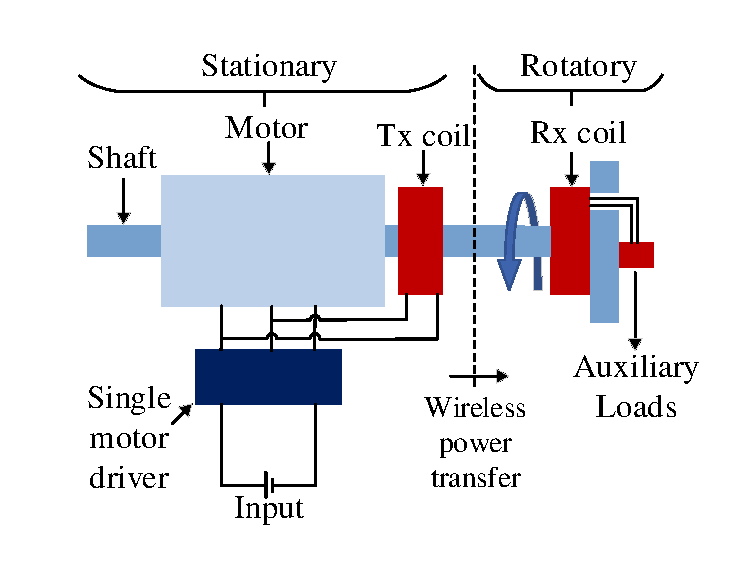
\includegraphics[width=0.30\linewidth]{new.pdf}}
    \hfill
    \subfigure[]{
    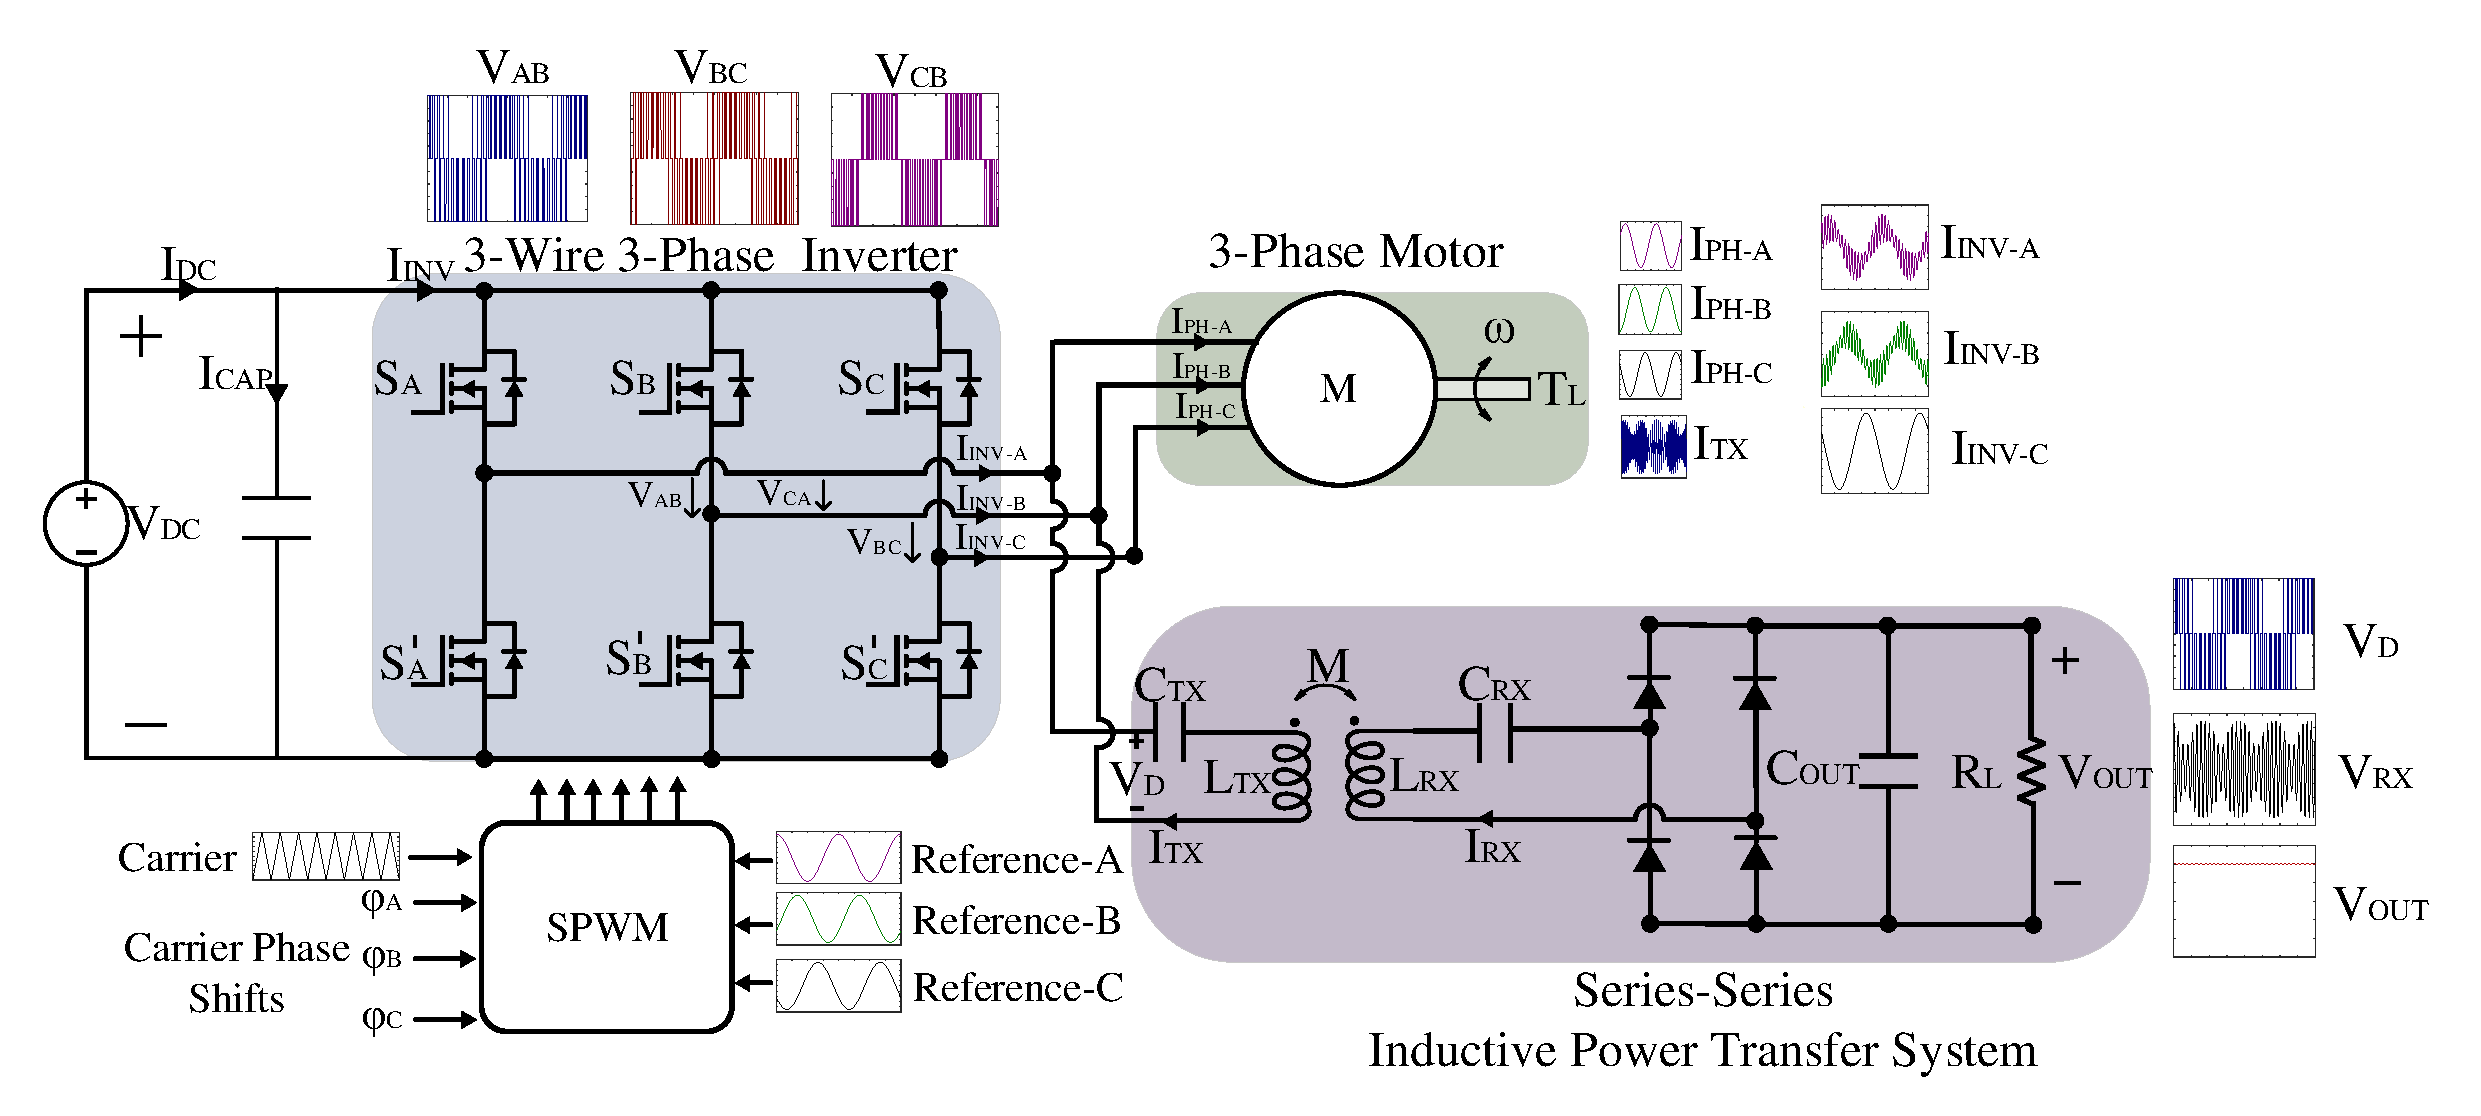
\includegraphics[width=0.66\linewidth]{system_proposal_3VSC_v2.pdf}}
    \caption{a) The proposed single-inverter multi-frequency motor drive and WPT system to energize IoT devices or sensors on the rotating frames. b) The circuit diagram of a single inverter system, which drives concurrently  $3W$-$3\Phi$ motor and WPT system.}
    \label{fig:Circuit-diagram}
\end{figure*}
%%%%

In this study,  a motor and an auxiliary system are driven concurrently by a single converter, as shown in Fig. \ref{fig:Circuit-diagram}.a. 
It is proposed that the already existing inverter of the drive can be used as a multi-frequency inverter; thus, the high-frequency converter of the WPT system can be eliminated, reducing the cost and complexity. 
Since the power rating of an auxiliary system is lower than the motor, the existing motor drive can also be used as a single inverter of a multi-frequency system.
Furthermore, conventional motor drives use several pulse width modulation (PWM) techniques (such as sinusoidal PWM, space vector PWM, and discontinuous PWM) to adjust the speed and torque of the motor.
However, independent control of the WPT system cannot be achieved only using these techniques. 
In this paper, a novel carrier phase shift (CPS) method is proposed, which provides independent control of the dual-band output voltage. 

The rest of the paper is organized as follows. 
Section~\RomanNumeralCaps{2} presents the modulation methods and the proposed CPS method. 
Section~\RomanNumeralCaps{3} delivers the design stage of the WPT system.
Section~\RomanNumeralCaps{4} explains the independent control of the motor and the WPT system.
Section~\RomanNumeralCaps{5} gives experimental results to validate the theoretical calculations.
Section~\RomanNumeralCaps{6} compares the proposed system with existing studies in the literature. 
Section~\RomanNumeralCaps{7} discusses the implementation of the proposed system to conventional industrial drives.


\section{System Proposal and Modulation Method}
A 3-phase 3-wire ($3\Phi$-$3W$) motor and a WPT system for auxiliary rotating loads are driven by a single inverter with sinusoidal PWM (SPWM) as a proof-of-concept.
The circuit diagram of the system and the expected voltage and current waveforms are shown in Fig. \ref{fig:Circuit-diagram}.b.
In this section, the analytical modeling of applied SPWM will be investigated. Then, the carrier phase shift (CPS) method is proposed, and the effect of this method on the magnitude of the dual-band output will be examined. Finally, the equivalent centered harmonic approach to control the amount of CPS is presented. 

\subsection{Analytical analysis of  SPWM}
SPWM is established by comparing a high-frequency triangular carrier signal and a fundamental (modulating) signal. 
This fundamental signal is the reference signal of the motor, and the operating frequency of WPT is cultivated using the first harmonic of the carrier signal.
The analytical model of SPWM can be obtained as given in (\ref{eq:double_fourier}), using double Fourier analysis.
\begin{equation}
\label{eq:double_fourier}
 \begin{split}
S&= \frac{1}{2}+ \frac{m_a}{2}\cos{\Big( \omega_ot+\theta_o\Big)}  \\
&+\frac{2}{\pi}\sum_{i=1}^{i=\infty}J_o\Big( i\frac{\pi}{2}m_a\Big)\sin{\Big(i\frac{\pi}{2}\Big)}\cos{ \Big( i(\omega_ct+\theta_c) \Big)}  \\
&+ \frac{2}{\pi}\sum_{i=1}^{i=\infty}\sum_{k=-\infty}^{k=\infty} 
  \Bigg(  \begin{array}{cc}
 \frac{1}{i} J_k\Big(i\frac{\pi}{2}m_a\Big)  \sin\Big((i+k)\frac{pi}{2}\Big)  \\
     \cos{\Big( i(w_ct+\theta_c) +k(w_ot+\theta_o) \Big)}
\end{array}\Bigg)
\end{split}
\end{equation}
There are four main components for each leg: DC, fundamental, switching harmonics, and sidebands.
The magnitudes of switching harmonics and their sidebands cannot be adjusted independently, and they change along with the modulation index, which is used to control the magnitude of the fundamental frequency.
\begin{figure}[h]
\centering
     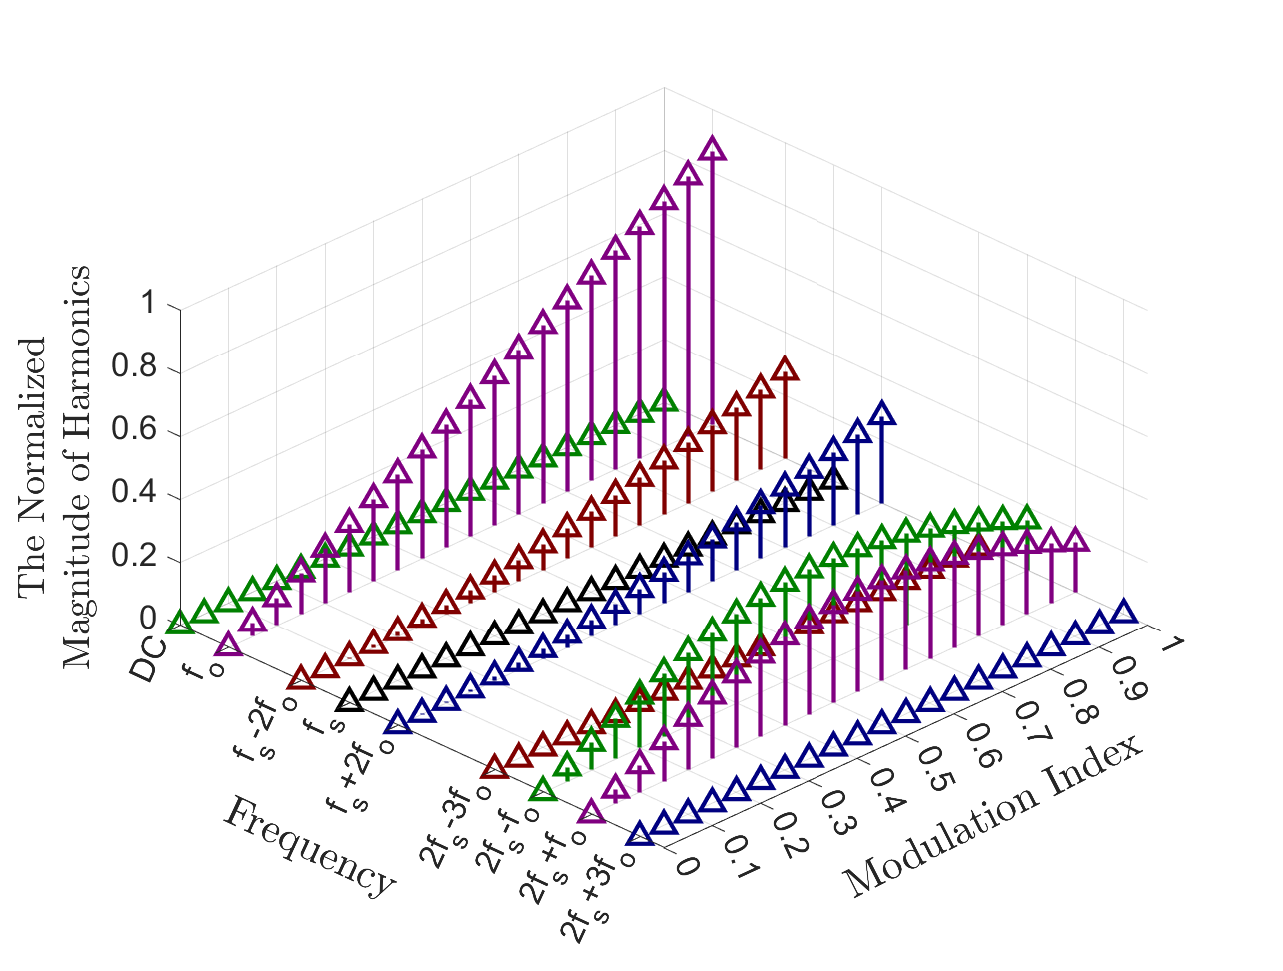
\includegraphics[width=0.8\linewidth]{harmonic_dist_VAB.eps}
  \caption{ The harmonic distribution of a line-to-line voltage among different modulation indices without carrier phase shift. (Their peak voltages per DC-link voltage are presented.)}
    \label{fig:harmonic_dist_VAB}
\end{figure}
Moreover, the phases of these components vary for each leg of the inverter, and they have positive, negative, or zero sequences, as shown in Table \ref{tab:zero_carrier_harmonics}.
The normalized line-to-line voltage harmonics are given in Fig. \ref{fig:harmonic_dist_VAB}.

\begin{table}[h]
\centering
\caption{The sequences of the fundamental frequency, switching harmonic, and its sideband harmonics}
\begin{tabular}{l|cccl}
\textbf{Frequency}   & \textbf{Leg A   }        & \textbf{Leg B  }       & \textbf{Leg C}    & \textbf{Sequence} \\ \hline \hline
$\mathrm{f_o} $       &     $ 0^o $          & $ 120^o $        & $ -120^o $      & Positive      \\ 
$\mathrm{f_s-2f_o }$  &     $ 0^o $          & $ 120^o $        & $ -120^o $      &  Positive     \\ 
$\mathrm{f_s}  $      &     $ 0^o $          & $ 0^o $          &  $ 0^o $        &  Zero         \\ 
$\mathrm{f_s+2f_o} $  &     $ 0^o $          & $ -120^o $       &  $ 120^o $      & Negative       \\ 
\end{tabular}
\label{tab:zero_carrier_harmonics}
\end{table}

Since the switching harmonic is zero-sequence, it disappears in a line-to-line connection, which means that the line-to-line connected WPT system is excited only by the sideband components. 
Additionally, the magnitude of these sideband components cannot be controlled independently. 
Therefore, in order to regulate the WPT power, a DC-DC converter can be added to the receiver for post-regulation, which increases cost and complexity.
Furthermore, this regulation method cannot guarantee to transfer power under each modulation index since sideband components converge to zero as $m_a$ comes up to zero. 
In other words, the transferred power of the WPT system is decreasing while $m_a$ is nearing zero.
This diminished power is undesirable since the auxiliary loads may require the rated power for each operating condition of the motor. 
 %%%%%%
\vspace*{-4mm}
\subsection{The Proposed Carrier Phase Shift (CPS) Method}
Normally, the power transmitted to the WPT system cannot be controlled independently for every $ m_a$ value  due to the non-controllable magnitude of sidebands and the disappearance of the switching frequency in the line-to-line connection.
It is proposed that these problems can be solved by giving a phase shift between carrier signals of two legs. As can be seen from the double Fourier analysis in (\ref{eq:double_fourier}), phases of switching frequency and its sidebands change as a function of the phase of the carrier signal. 
In this study, for the coherency,  the WPT system will be connected between legs A and B, and a carrier phase shift will be given to leg B, as given in (\ref{eq:Phi}).
\begin{equation}
\label{eq:Phi}
Carrier \ phases 
 \begin{cases}
      \phi_{cA}= 0\\
       \phi_{cB}= \phi_{CPS}\\
      \phi_{cC}= 0
\end{cases}    
\end{equation}
% \vspace{-4mm}
\begin{figure}[h]
\centering
     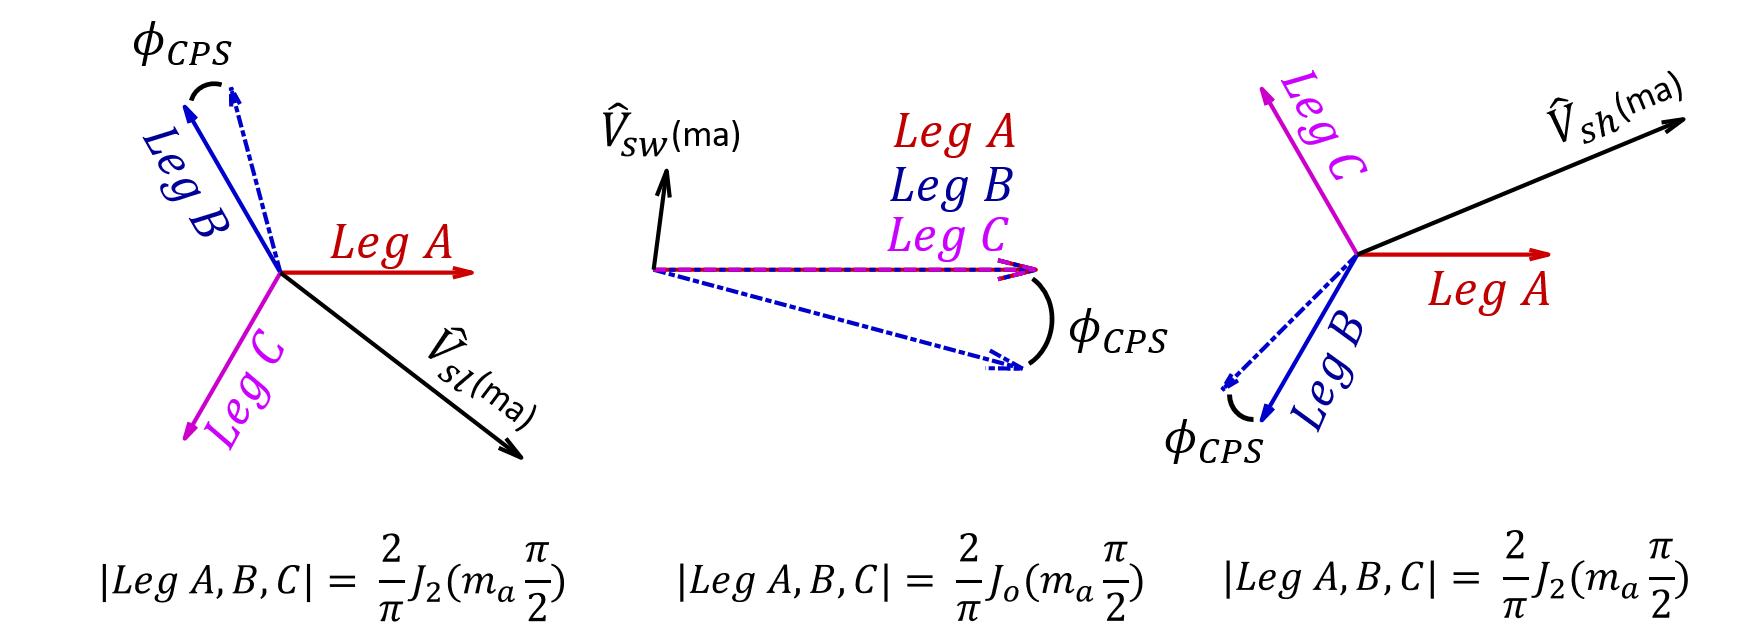
\includegraphics[width=1\linewidth]{phasor.png}
  \caption{ Phasor diagram of the switching frequency and sideband harmonics.}
    \label{fig:phasor}
\end{figure}
\begin{figure*}[t!]
\centering
\subfigure[]{
    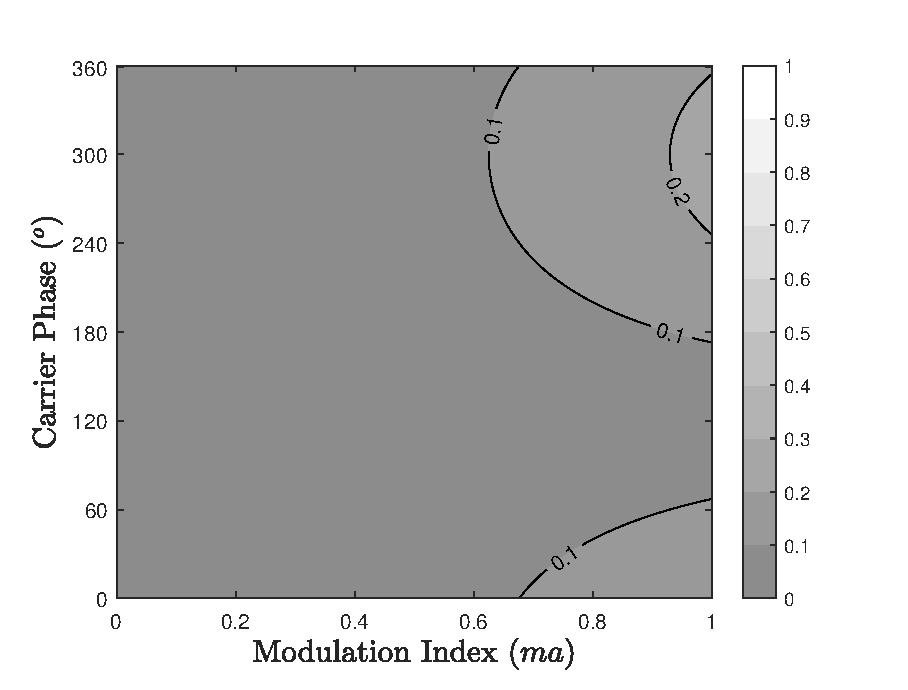
\includegraphics[width=0.31\linewidth]{control_space_fl1.eps}
    }
\subfigure[]{
    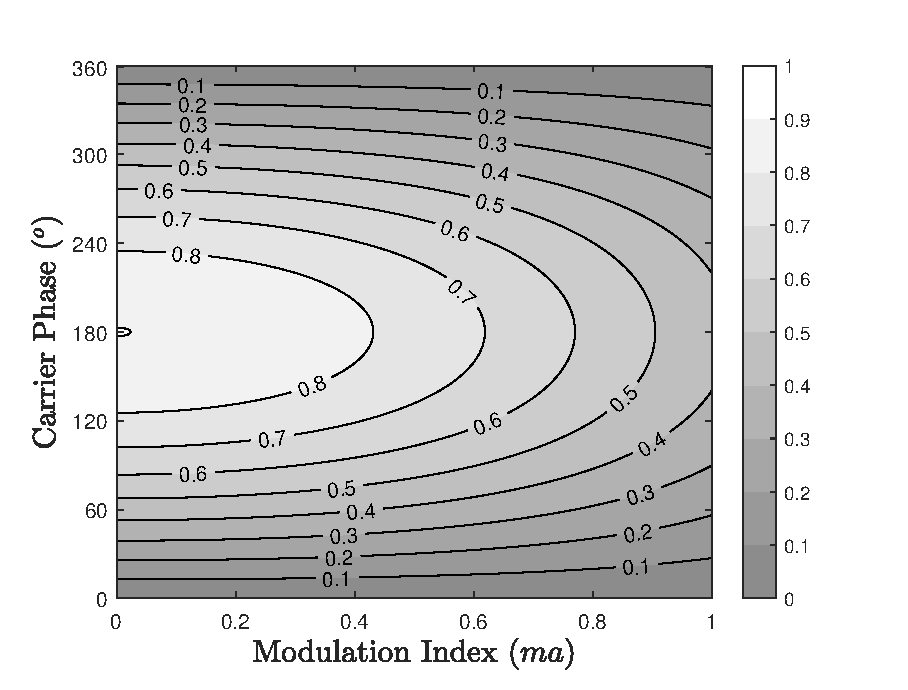
\includegraphics[width=0.31\linewidth]{control_space_fsw1.eps}
    }
\subfigure[]{
    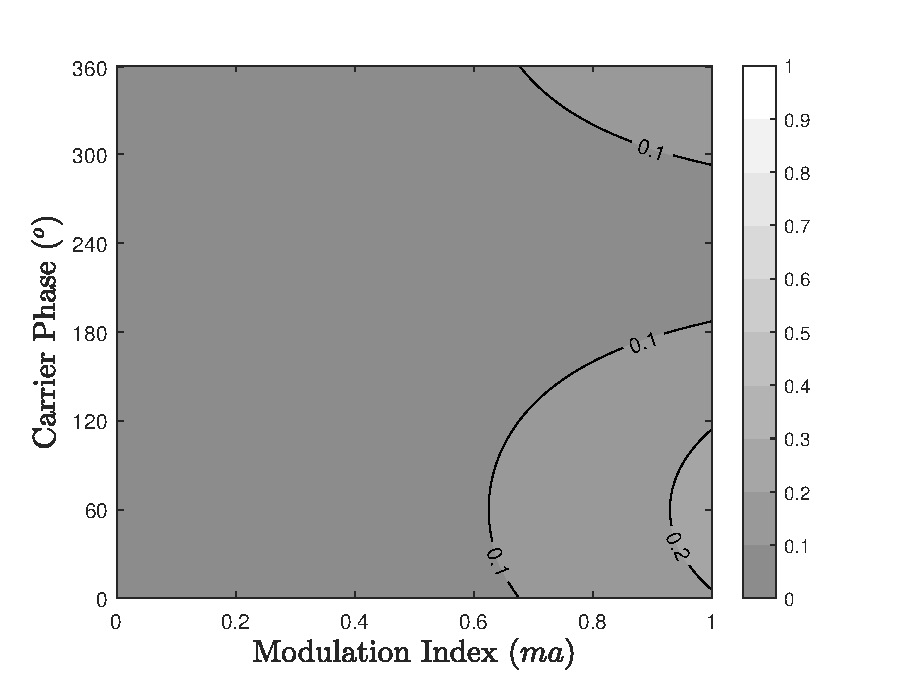
\includegraphics[width=0.31\linewidth]{control_space_fh1.eps}
    }
        \caption{Normalized inverter ouput voltages $|\frac{V_{l-l}}{V_{DC}}|$. 
        (a) Lower sideband of the switching frequency ($\mathrm{f_{sl}}$). 
        (b) Switching frequency ($\mathrm{f_{s}}$).
        (c) Higher sideband of the switching frequency ($\mathrm{f_{sh}}$).}
    \label{fig:control_space}
\end{figure*}

The phasor diagram of the switching frequency and sideband harmonics for each leg are represented in Fig. \ref{fig:phasor}.
The magnitude of these components can be calculated as in (\ref{eq:double_fourier}) by taking $(i=1)$, $(i=1,k=-2) $, and $(i=1,k=2)$.
The harmonic components between phase A and phase B, the magnitudes of which can be calculated via phasor subtractions, can be controlled by the carrier phase shift of phase B. 
Thus, the magnitudes of these components can be calculated as given in (\ref{eq:sl_M}, \ref{eq:sw_M}, \ref{eq:sh_M}).

\newpage

\begin{equation}
\label{eq:sl_M}
\hat{V}_{sl}(m_a)=\frac{2}{\pi} J_2\bigg(m_a\frac{\pi}{2}\bigg)\sqrt{1-cos(\phi_{CPS}+120^o)}  
\end{equation}
\begin{equation}
\label{eq:sw_M}
\hat{V}_{sw}(m_a)= \frac{2}{\pi} J_o\bigg(m_a \frac{\pi}{2}\bigg)\sqrt{1-cos(\phi_{CPS})}  
\end{equation}
\begin{equation}
\label{eq:sh_M}
\hat{V}_{sh}(m_a)=\frac{2}{\pi} J_2\bigg(m_a\frac{\pi}{2}\bigg)\sqrt{1-cos(\phi_{CPS}-120^o)}  
\end{equation}

The magnitudes are calculated for variable carrier phase shifts and modulation indices, as shown in Fig. \ref{fig:control_space}. A challenge is to determine the amount of the phase shift, which must guarantee constant power transfer for any modulation indices. Since the magnitudes of switching frequency harmonic and sidebands change differently, a combined equivalent magnitude value is required to select the amount of phase shift.
 
\subsection{Equivalent centered harmonics approach}
Considering the quality factor of WPT systems, the gain of the switching frequency and its sideband harmonics are nearly equal since their frequencies are close enough. Instead of investigating each component in the time domain, we can build an equivalent drive voltage assuming all components have the same frequency.
These components generate power, which is dissipated on the $R_L$. The same dissipated power on the $R_L$ can be produced by an equivalent drive voltage ($V_D$). Using the power equality in  (\ref{eq:equ_cent1}),  ($V_D$) is calculated as given in (\ref{eq:equ_cent}).
%%%
\begin{equation}
\label{eq:equ_cent1}
P_{R_L}=\frac{V_{D}^2}{R_L}=\frac{V_{sl}^2}{R_L} +\frac{V_{sw}^2}{R_L} +\frac{V_{hl}^2}{R_L} 
\end{equation}
%%%%
\begin{equation}
\label{eq:equ_cent}
V_{D}=  \sqrt{\bigg(V_{sl}^2+V_{sw}^2+V_{sh}^2 \bigg)}
\end{equation}
%%%%
Using the equivalent center harmonic approach, a normalized drive voltage is shown for various carrier phase shifts and modulation indices in Fig. \ref{fig:control_space_center}. 
For each modulation index, we can guarantee the normalized gain between 0.28 and 0.45 by adjusting the carrier phase shift. 
However, if a higher gain is required, the modulation index of the motor drive should be restricted to achieve this gain for all conditions, which narrows the operation region of the motor. 
Therefore, the normalized gain is selected considering the DC-link voltage, motor modulation index requirements, output voltage, and output power of the WPT system.
\begin{figure}[h!]
\centering
    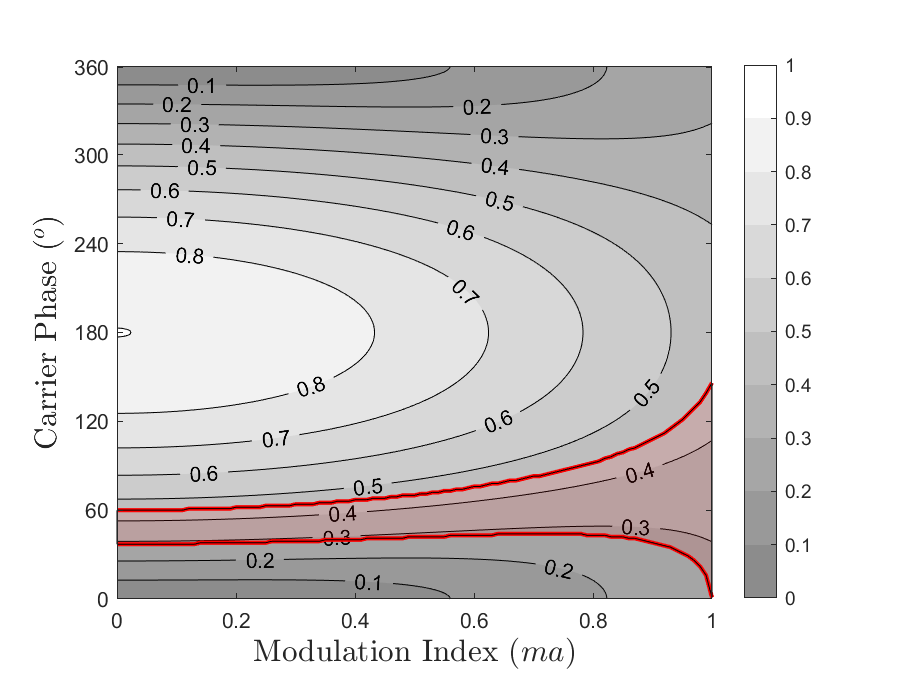
\includegraphics[width=0.8\linewidth]{control_space_fall_restricted.eps}        
    \caption{ Normalized inverter output voltages $|\frac{V_{l-l}}{V_{DC}}|$ using the center harmonic approach. The constant drive voltage gains, which can be achieved in any modulation index, are colored red.}
    \label{fig:control_space_center}
\end{figure}
%%%%%%%%%%%%%%%
\section{WPT System Parameters Specification}
As a proof of concept, the WPT system is implemented with a 100 V DC-link and switching frequency up to 100~kHz. 
The system is designed to energize auxiliary systems, so constant voltage (CV) output is required. The output voltage and rated power of the WPT system are given in Table \ref{tab:WPT_ratings}. 
The circuit diagram of the series-series compensated WPT system is shown in Fig. \ref{fig:WPT_system}. 
\begin{figure}[h!]
    \centering
    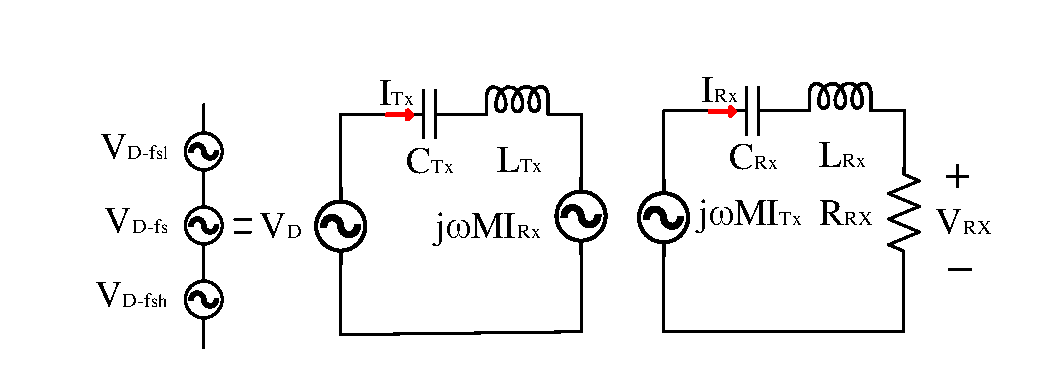
\includegraphics[width=1\linewidth]{FHA.pdf}
    \caption{The first harmonic approach circuit diagram of the WPT system.}
    \label{fig:WPT_system}
\end{figure}
%%%%%%%%
\begin{table}[h!]
\centering
\caption{The Input-Output Specifications of the WPT System}
\label{tab:WPT_ratings}
%%%%%%%%%
\begin{tabular}{ll}
\textbf{Ratings}  &    \\ \hline
DC-link Voltage ($V_{DC}$)    & $\mathrm{100~V}$ \\
Modulation Index  ($m_a$)  & $\mathrm{0-1}$ \\
Switching frequency  ($f_s$)  & $\mathrm{<100kHz}$ \\
Output Voltage    ($V_{OUT}$)   & $\mathrm{15~V}$ \\
Rated Power      ($P_{rated}$)     & $\mathrm{30~W}$ \\
\hline
\hline
\\
\textbf{Design Parameters}  &    \\ \hline
Receiver voltage ($V_{Rx}$) & $\mathrm{16.7~V_{RMS}}$ \\
Gain of the WPT System  ($A_{WPT}$)  & $\mathrm{0.5}$ \\
WPT Input Voltage  ($V_{D}$)  & $\mathrm{33.4~V_{RMS}}$ \\
Normalized Drive Voltage   & $\mathrm{0.334}$ \\
\end{tabular}
\end{table}
%%%%%%%%%

Since the output voltage is 15~V,  for SS-compensated system, the receiver voltage is 16.7 $V_{RMS}$ as can be calculated in  $V_{RX} =  V_{OUT}\frac{2\sqrt{2}}{\pi}$.
The motor operates under the full range of modulation index (0-1); thus, the normalized drive voltage should be selected between 0.28 and 0.45 to avoid modulation restriction.
The gain of the WPT system is selected as 0.5, which means that the input voltage should be 33.4 $V_{RMS}$, and the normalized drive voltage becomes 0.334.
%%%%%%%
For SS compensation, the frequency of the  CV operation (or as known as load-independent voltage) is different from the resonant frequency ($w_r$), and there are two operating frequencies ($\omega_{rl}, \omega_{rh}$).
The receiver voltage ($V_{RX}$) and voltage gain ($A_{WPT}$) of the SS compensated system are given in (\ref{eq:Vout}) and~(\ref{eq:Awpt}). 
%%%%%%
\begin{equation}
\label{eq:Vout}
    V_{RX} =  \frac{j\omega M I_{Tx}}{Z_{Rx}}R_L  = \frac{j\omega M V_{D}}{\omega^2M^2+Z_{Tx}Z_{Rx}}R_L
\end{equation}
%%%%%%%
\begin{equation}
\label{eq:Awpt}
    A_{WPT} =  \bigg|\frac{V_{RX}}{V_{D}}\bigg| = \frac{\omega M}{\omega^2M^2+Z_{TX}Z_{RX}} R_L
\end{equation}
%%%%%%%
In order to calculate the frequencies providing load-independent voltage gain, the differential equation of $\frac{dA_{WPT}}{d  R_L} =0$ should be solved \cite{CV}. 
The load-independent voltage operating frequencies are found as in (\ref{eq:CV_freq}) according to selected coupling factor ($k$) and angular resonant frequency~($w_r$).
%%%%%%%%%%%%%%%
\begin{equation}
\label{eq:CV_freq}
    \omega_{rl,rh} =  \omega_r \sqrt{\frac{1}{1 \pm k}} 
\end{equation}
%%%%%%%%%%
The minimum load resistance that delivers the rated power can be calculated as in (\ref{eq:R_L}). 
\begin{equation}
\label{eq:R_L}
   R_L= \frac{V_{RX}^2}{P_{rated}}
\end{equation}
Receiver inductance is calculated using the load resistance, operating frequency that is selected as $w_{rh}$, and the chosen quality factor of Rx ($Q_{Rx}$) as provided in (\ref{eq:L_RX}). 
\begin{equation}
\label{eq:L_RX}
\begin{split}
     Q_{Rx}= \frac{\omega_{rh}L_{Rx}}{R_L} 
\end{split}
\end{equation}
%%%%%%%%
The load-independent voltage gain is presented in (\ref{eq:AWPT_wr}), and the Tx inductance is found using (\ref{eq:L_Tx}). 
%%%%%%%
\begin{equation}
\label{eq:AWPT_wr}
    A_{WPT(\omega_{rh})} = \bigg | \sqrt{\frac{L_{Rx}}{L_{Tx}}} \bigg |
\end{equation}
%%%%%%%%
\begin{equation}
    \label{eq:L_Tx}
   L_{Tx}= \frac{L_{Rx}}{ A_{WPT(\omega_{rh})}^2}
\end{equation}
%%%%%%%%
Then, the mutual inductance is calculated as in (\ref{eq:mutual}).
\begin{equation}
\label{eq:mutual}
   M= k\sqrt{L_{Tx}L_{Rx}}
\end{equation}
%%%%%%%%%
Finally, the compensation capacitances are adjusted as in (\ref{eq:C_txrx}).
\begin{equation}
\label{eq:C_txrx}
      C_{Tx,Rx} = \frac{1}{\omega_r^2L_{Tx,Rx}}
\end{equation}
%%%%%%%%%
The initial parameters and the derived parameters are given in Table \ref{tab:derived}. The operating frequency is selected 85~kHz, which provides a frequency control  region up to 100~kHz. 
$Q_{RX}$ is selected between 2-10 as a rule of thumb \cite{aditya}, and the coupling coefficient ($k$) is between 0 and 1. In this study,  $Q_{RX}$ and k are selected as 2.9 and 0.4, respectively.
%%%%%%%
\begin{table}[h]
\centering
\caption{WPT System Parameters}
\label{tab:derived}
\begin{tabular}{cc|cc}
\begin{tabular}{c} \textbf{Initial/Choosen} \\ \textbf{Parameters}   \end{tabular}     & \textbf{Values} &  \begin{tabular}{c} \textbf{Derived} \\ \textbf{Parameters}   \end{tabular}
&  \textbf{Values}  \\
\hline
$\mathrm{P_{rated}}$  & \30~W  & $ \mathrm{R_L}$ & 9.3 $\Omega $\\
$\mathrm{V_{D}}$ & $33.4~V_{RMS}$ &   $\mathrm{L_{Rx}}$    & 50~$\mu H$\\
$\mathrm{V_{OUT}}$ & $15~V$ &  $\mathrm{L_{Tx}}$ & 200~$\mu H$ \\
$f_{rh}$ & 85~kHz &     $\mathrm{M}$ & 40~$\mu H$ \\
$Q_{Rx}$  & 2.9  &  $\mathrm{f_{r}}$  &  65.85~kHz  \\
$k$ & 0.4 &  $\mathrm{C_{Tx}}$  &   29.2~nF \\
$\mathrm{V_{RX}}$ & $16.7~V_{RMS}$ & $\mathrm{C_{Rx}}$  &   117~nF \\
 $ \mathrm{A_{WPT}}$ & 0.5 &  &    \\
\hline
\end{tabular}
\end{table}
%%%%%%%%
\section{Control Scheme of WPT System}
The carrier phase shift is introduced to keep the $V_D$ constant under varying modulation indices. 
It is observed that the carrier phase shift has narrow control region since the normalized gain of $V_D$ per unit DC-link voltage is restricted between 0.28 and 0.45 to operate under any modulation index. 
Since the system requires a constant voltage output, and the WPT system operates at the frequency of the load-independent voltage, a look-up table can be implemented to keep $V_D$ constant. 
However, minor variations in the output voltage due to parasitic effects or disturbances can occur. 
Therefore, additional frequency detuning control can be implemented to regulate  $V_D$. 
The overall control scheme is presented in Fig.~\ref{fig:control}.
\begin{figure}[h!]
    \centering
    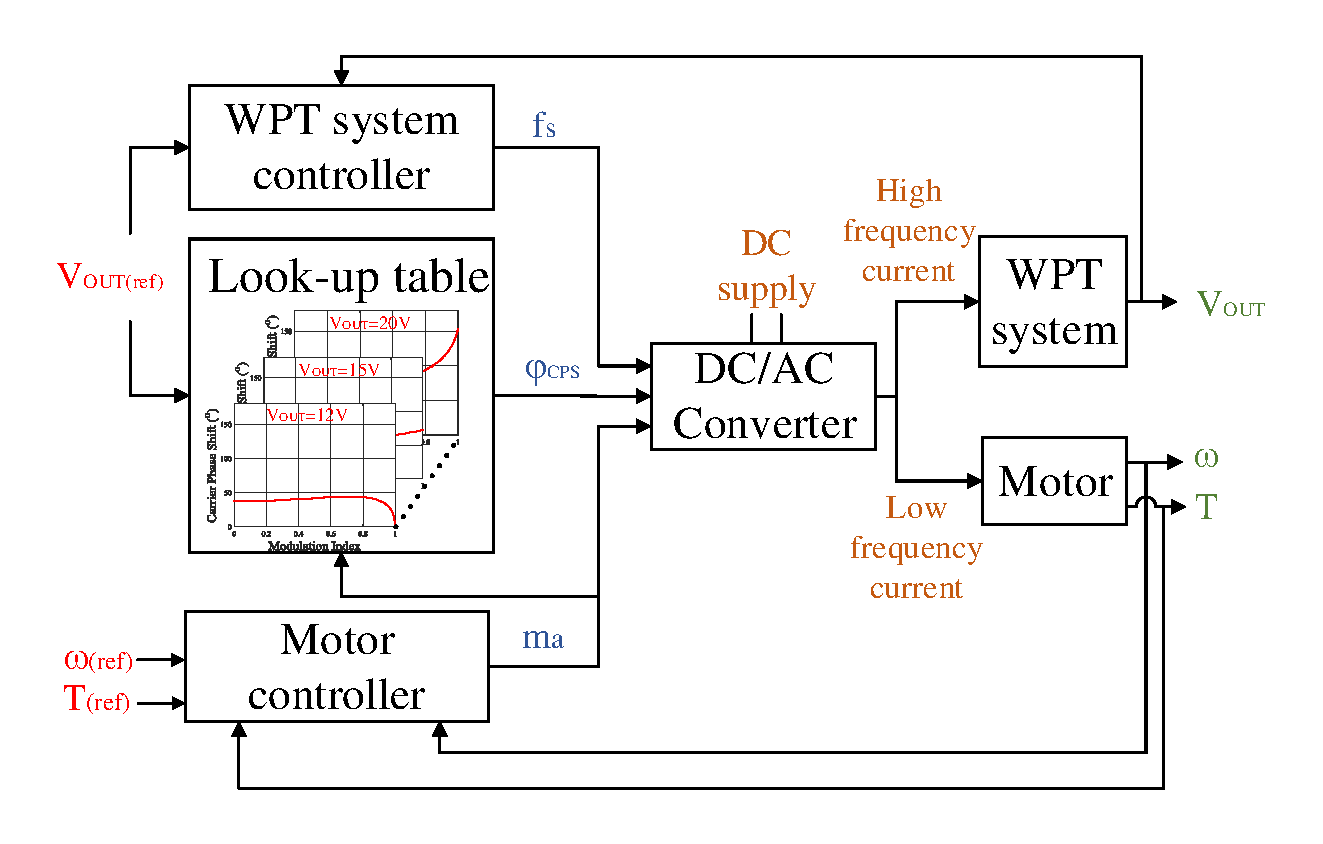
\includegraphics[width=1\linewidth] {Controller3AC_v3.pdf}
    \caption{Control algorithm of the combined carrier phase shift and frequency detuning method.}
    \label{fig:control}
\end{figure}
%%%%%%%%%
\section{Experimental Validation}
An experimental setup is established consisting of a GaN-based $3\Phi$-$3W$ inverter and an AC motor to validate the proposed method. The experimental setup is shown in Fig.~\ref{fig:exp_setup}. The AC motor is loaded using a DC generator, and the WPT system is connected to its shaft.
%%%%%%%%%
\begin{figure}[h!]
    \centering
    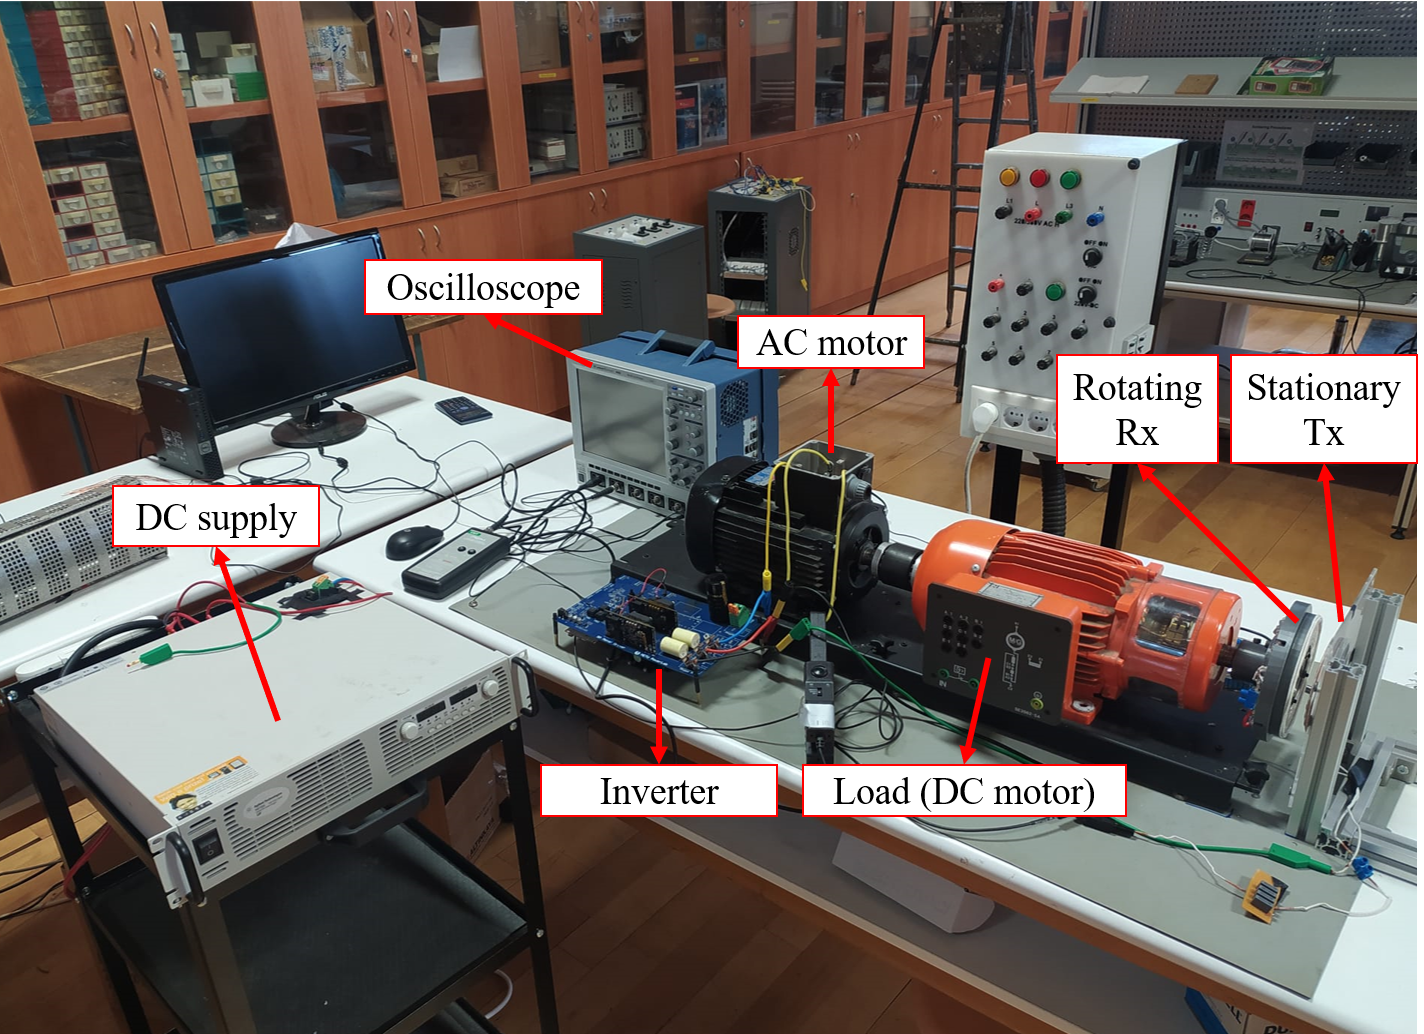
\includegraphics[width=0.8\linewidth]{setup2.png}
    \caption{Experimental Setup.}
    \label{fig:exp_setup}
\end{figure}
%%%%%%%%%
\vspace*{-5mm}
\subsection{Multi-frequency Inverter Test}
In this part, the inverter is driven by the SPWM modulation technique with and without the proposed CPS method.
Thus, the variation in the magnitudes of the fundamental frequency, switching frequency, and its sidebands are investigated.

The inverter output voltages are shown in Fig.~\ref{fig:multi-freq}  for the phase shift of $\phi_B=0^o$ and $\phi_B=47.5^o$.
The harmonic distributions of the normalized inverter output voltage are compared in Table \ref{tab:multi-freq} for analytical and experimental results, which have a good agreement with an error band of less than 10\%.
It can be observed that the carrier phase shift method controls the magnitude of the switching frequency component and its sidebands while the magnitude of the fundamental component stays constant.
\begin{table}[h]
\caption{Theoretical and experimental results of inverter output harmonic distribution for $\phi_{CPS}=0^o$ and $\phi_{CPS}=47.5^o$ }
\label{tab:multi-freq}
\centering
\begin{tabular}{lc|llll}

\multicolumn{2}{l}{\multirow{2}{*}{}}  &  & \multicolumn{3}{l}{$A_{INV}$ ($\hat{V}_{ll}/V_{dc}$)}  \\  \cline{3-6}  % row1

\multicolumn{2}{l}{}&\multicolumn{1}{l}{at $\mathbf{f_o}$}&\multicolumn{1}{l}{at $\mathbf{f_l}$}& \multicolumn{1}{l}{at $\mathbf{f_s}$}& \multicolumn{1}{l}{at $\mathbf{f_h}$} \\ \cline{1-6}  % row 2

\multicolumn{1}{l|}{\multirow{3}{*}{\begin{tabular}[c]{@{}l@{}}$\mathbf{m_a=0.6}$\\ $\mathbf{\phi_{CPS}=0}$\end{tabular}}}    & \textbf{
    Theoretical} & \multicolumn{1}{l|}{0.519} & \multicolumn{1}{l|}{0.113}  & \multicolumn{1}{l|}{0}     & 0.113 \\ \cline{2-6}  % row 3

\multicolumn{1}{l|}{}  & \textbf{
   Experimental  } & \multicolumn{1}{l|}{0.532} & \multicolumn{1}{l|}{0.110}  & \multicolumn{1}{l|}{0.011} & 0.115 \\ \cline{2-6}  % row4

\multicolumn{1}{l|}{}   & \textbf{Error }     & \multicolumn{1}{l|}{2.5\%} & \multicolumn{1}{l|}{2.6\%} & \multicolumn{1}{l|}{-} & \multicolumn{1}{l}{1.7\%} \\ \hline % row5

\multicolumn{1}{l|}{\multirow{3}{*}{\begin{tabular}[c]{@{}l@{}}$\mathbf{m_a=0.6}$\\ $\mathbf{\phi_{CPS}=47.5^o}$\end{tabular}}} & \textbf{
    Theoretical }& \multicolumn{1}{l|}{0.519} & \multicolumn{1}{l|}{0.130}  & \multicolumn{1}{l|}{0.405} & 0.077 \\ \cline{2-6}  % row6

\multicolumn{1}{l|}{}   &\textbf{
   Experimental }& \multicolumn{1}{l|}{0.537} & \multicolumn{1}{l|}{0.127}  & \multicolumn{1}{l|}{0.414} & 0.084 \\ \cline{2-6} % row7

\multicolumn{1}{l|}{}  & \textbf{Error }     & \multicolumn{1}{l|}{3.4\%} & \multicolumn{1}{l|}{2.3\%} & \multicolumn{1}{l|}{2.2\%} & \multicolumn{1}{l}{9.1\%} \\ \hline % row8
\end{tabular}
\end{table}
%%%%%%%%%
\begin{figure}[h]
\centering
\subfigure[$\phi_{CPS}=0^o$]{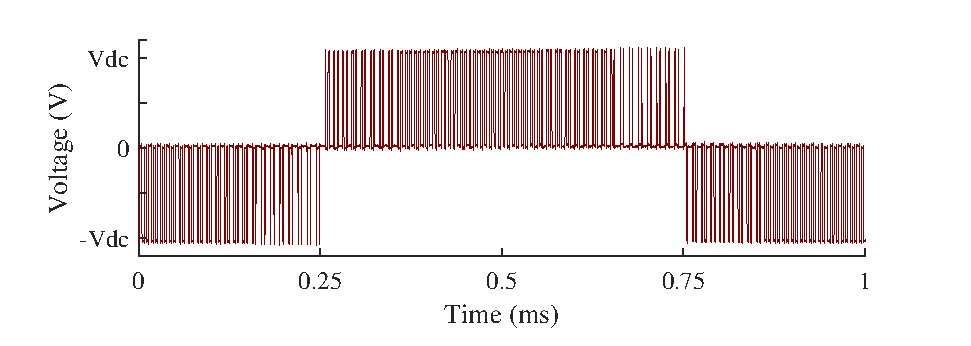
\includegraphics[width=1\linewidth]{m0.6_0_v2.eps}}
\subfigure[$\phi_{CPS}=47.5^o$]{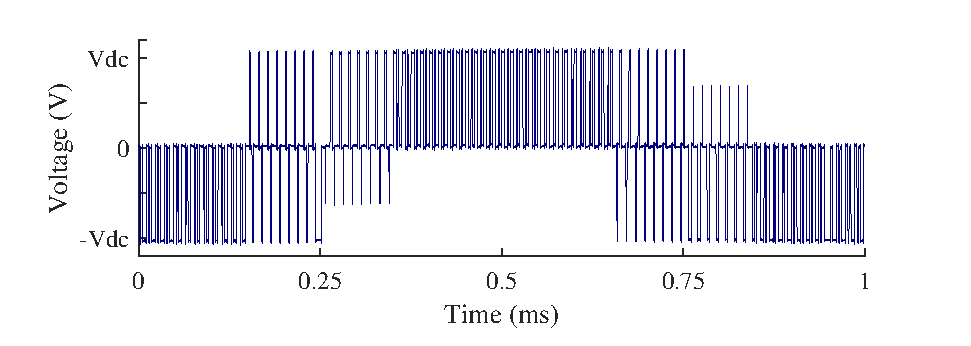
\includegraphics[width=1\linewidth]{m0.6_47_v2.eps}} 
 \caption{Inverter output voltage ($V_{l-l}$) (or called as drive voltage $V_{D}$ ) at $m_a =0.6$ for $\phi_{CPS}=0^o$ and $\phi_{CPS}=47.5^o$}
    \label{fig:multi-freq}
\end{figure}
%%%%%%%%%%
\vspace*{-5mm}
\subsection{Concurrent Operation of motor and WPT}
The motor and WPT system are driven standalone and concurrently. 
$CPS$, $f_s$, and $m_a$ are adjusted to  $50^o$, $82~kHz$, and $0.8$. 
Besides, the fundamental frequency of the motor is $20~Hz$.    
Firstly, the motor is operated standalone,  where the motor draws $1.58A$ as presented in Fig. \ref{fig:concurrent}.a.  
Then,  only the WPT system is connected, and its output voltage, Tx current, and Rx current are measured as given in Fig. \ref{fig:concurrent}.b.  
Finally, the motor and WPT system are run concurrently, and it is observed that the systems draw and supply almost the same current and voltage as shown in Fig. \ref{fig:concurrent}.c. 
It is observed that the output voltage differs by 1.7\%.
These minor changes stem from the varying effective duty cycle for the different converter currents due to the dead time duration.
It is also observed that a low-frequency fluctuation exists in the output voltage, which will be discussed in Section VII.
%%%%%%%%%%
\begin{figure}[h!]
\centering
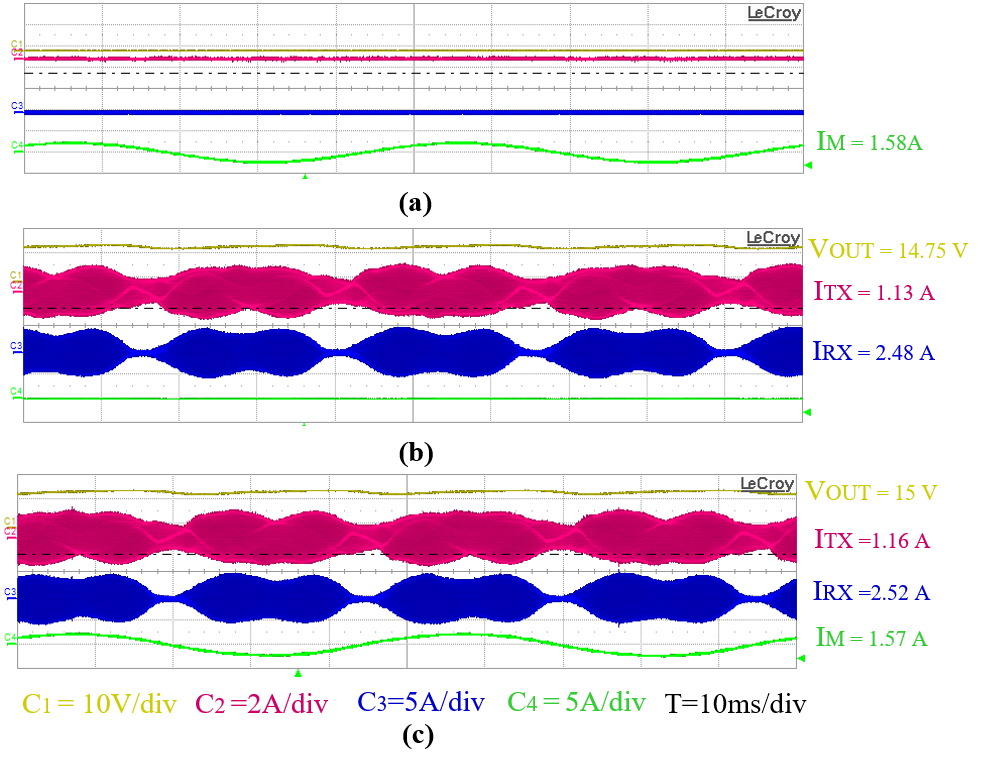
\includegraphics[width=1\linewidth]{concurrent_operation.png} 
\caption{ The waveforms of the DC output voltage, Tx current, Rx current, and motor current. a)  Standalone motor operation. b) Standalone WPT system operation. c) Concurrent operation.}
    \label{fig:concurrent}
\end{figure}
%%%%%%%%%
\vspace*{-5mm}
\subsection{Transient Load Changes of the Motor and the WPT System }
% \vspace*{-1mm}
In this part, the effect of the load changes on the WPT system and motor is investigated.
Firstly,  the mechanical load of the AC motor is varied, while other parameters such as switching frequency and modulation index are kept constant. It is observed that the WPT system is not disturbed by the load changes, as shown in Fig \ref{fig:transients}.a. 
Then, the load of the WPT system is altered using the same procedure.
As expected, currents of the AC motor do not change, as shown in Fig.~\ref{fig:transients}.b.  
Unless the modulation index or switching frequency varies, load changes of a system do not affect the operation of the other system.
Furthermore, in Fig.  \ref{fig:transients}, it is observed that the Tx current has some high-order harmonics ( $3^{rd}$ and $5^{th}$ harmonics of the switching frequency). Since the mathematical model is developed using only switching frequency and its sideband harmonics, the output voltage deviates from the desired value if the theoretic carrier phase shift is applied.
The combined carrier phase shift and frequency detuning control method, which will be revisited in the following part F,  can compensate for this deviation.
%%%%%%%%
\vspace{-4mm}
\begin{figure}[h!]
\centering
\subfigure[At $t_1$, the motor load torque is increased, and at $t_2$, the motor load torque returns to the former value. ]{
    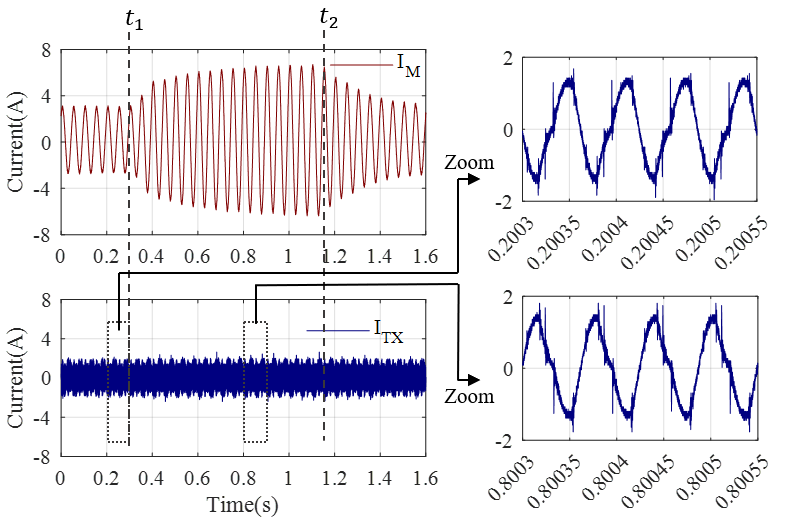
\includegraphics[width=0.83\linewidth]{motor_transients_v2.png}
    }
\subfigure[At $t_1$, The WPT load resistance is decreased, and at $t_2$, WPT load resistance returns to the former value.]{
    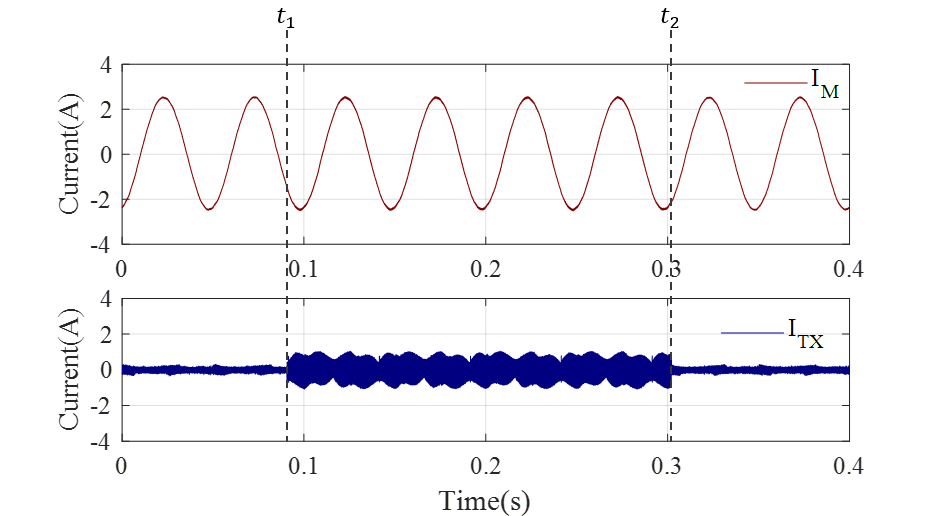
\includegraphics[width=0.83\linewidth]{WPT_transients_v2.png}
    }
        \caption{Transient load changes. a) Motor load changes. b) IPT load changes.}
    \label{fig:transients}
\end{figure}
%%%%%%%%%
% \vspace{-8mm}
\subsection{DC Output Reference Change and Fundamental Frequency Variation}
In this part, the effects of DC output reference change and fundamental frequency variation are investigated. Firstly, the carrier phase shift is adjusted to $44.5^o$ to achieve a 15 V DC output ($f_s$ is 80 kHz, $f_o$ is 10Hz, and $m_a$ is 0.36). The DC reference is decreased to 8 V by adjusting carrier phase shift to $23^o$, and then increased to 15 V DC. The DC output voltage, motor, Tx and Rx currents are shown in Fig. \ref{fig:transients_DC_references}.  It is observed that the motor current is not affected by this change.

%%%%%%%%
\begin{figure}[h!]
\centering
    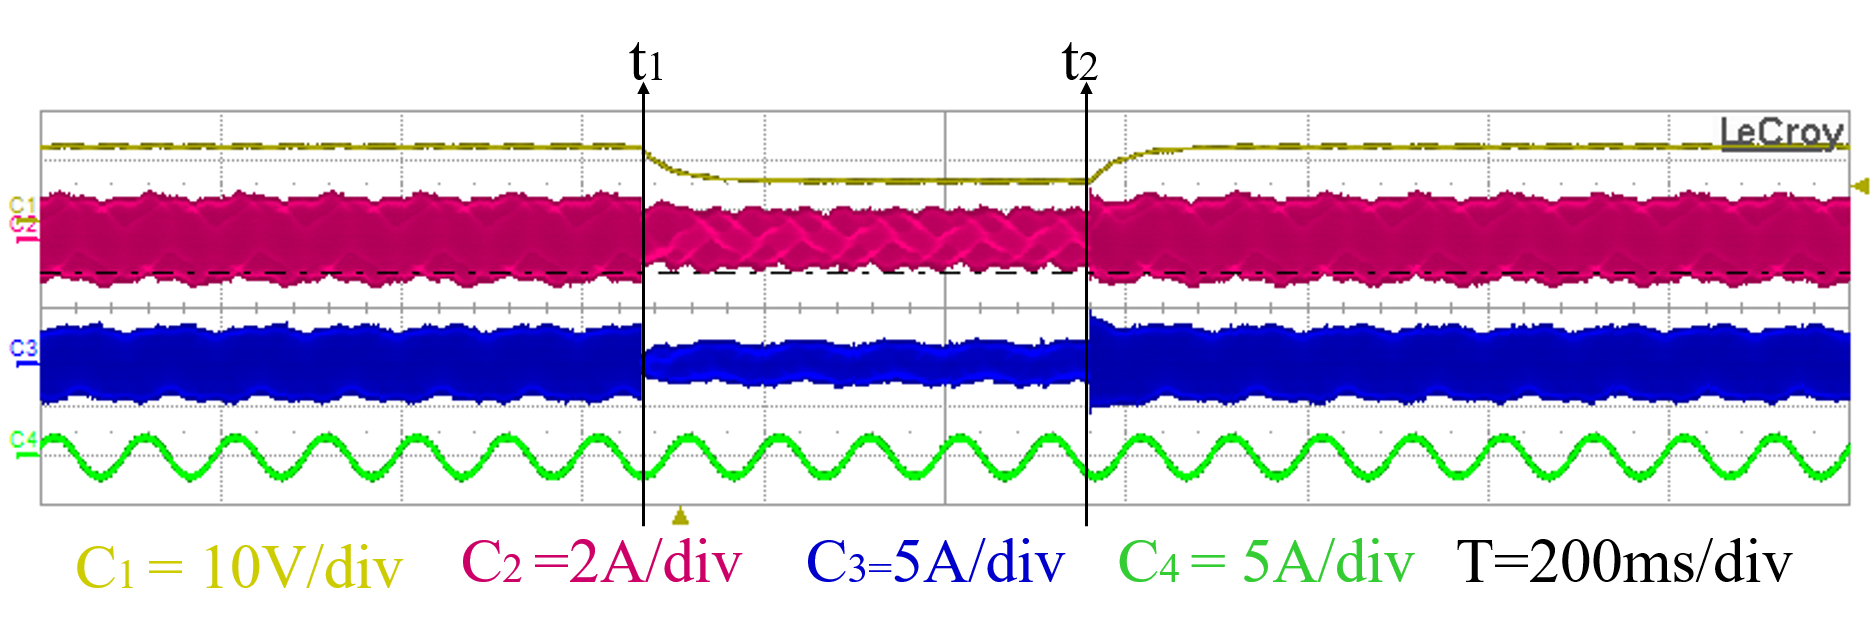
\includegraphics[width=1\linewidth]{DC_reference.png}
        \caption{ The current and voltage waveforms for DC reference changes.} 
    \label{fig:transients_DC_references}
\end{figure}
%%%%%%%%%%%
Secondly, a resistive-inductive (RL) load is connected to the motor drive, and the fundamental frequency is swept from 0 to 50 Hz. The carrier phase shift is adjusted to $44.5^o$ to achieve a 15 V DC output ($f_s$ is 80~kHz, and $m_a$ is 0.36). The current of the RL load and DC output voltage is shown in Fig. \ref{fig:transients_frequency}. It is observed that the DC output voltage is constant while the fundamental frequency is changing.

\begin{figure}[h!]
\centering
    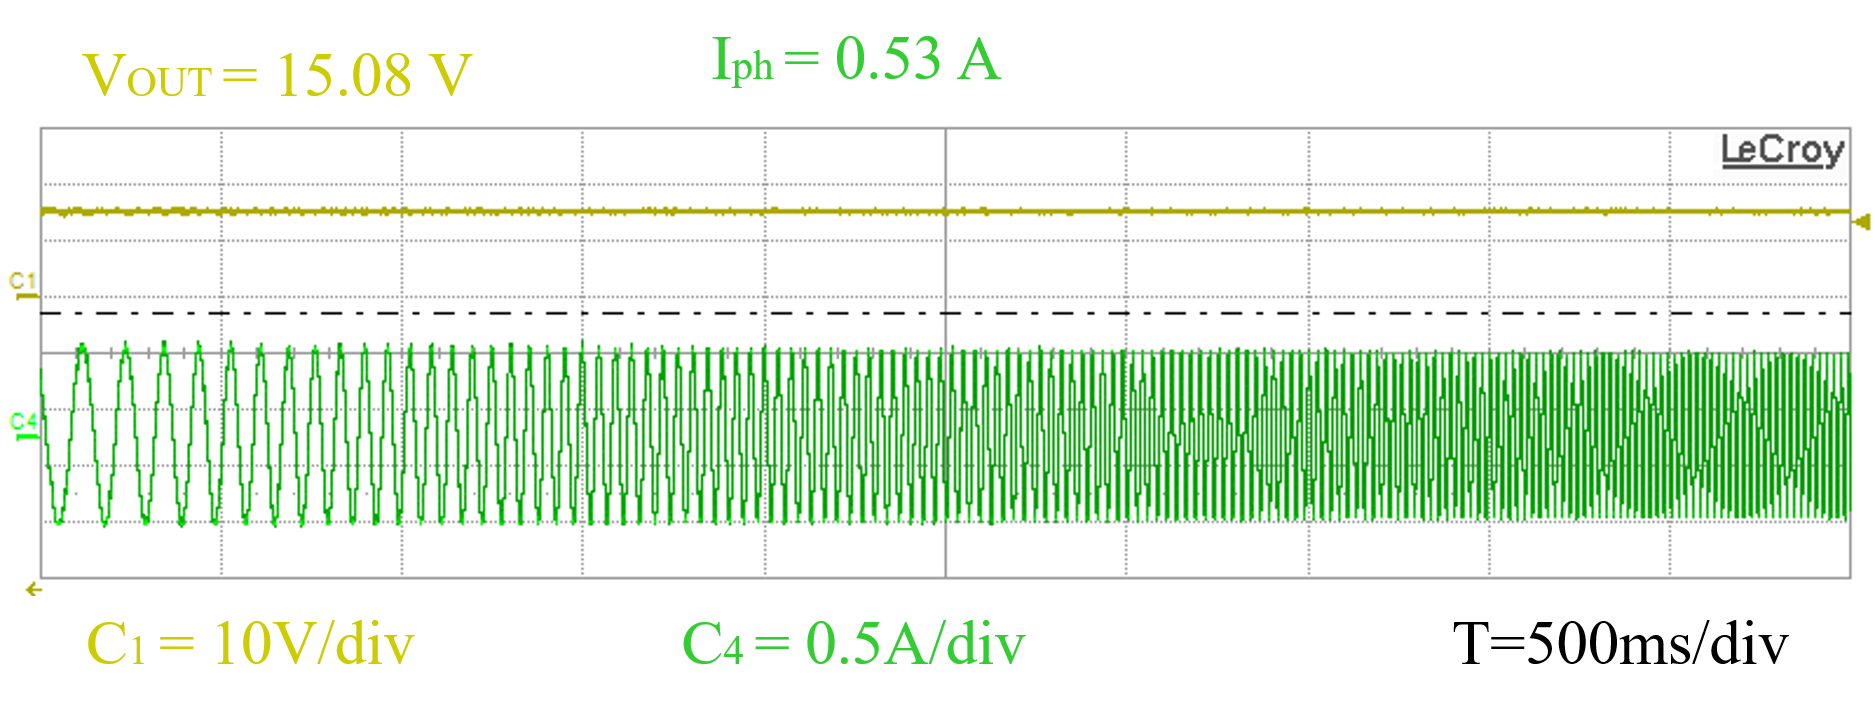
\includegraphics[width=1\linewidth]{fundamental_reference.png}
        \caption{ The output voltage and phase current under identical $m_a$ and $CPS$ for fundamental frequency variation between 0 to 50 Hz  } 
    \label{fig:transients_frequency}
\end{figure}
%%%%%%%%

\vspace*{-12mm}
\subsection{Efficiency and Drive Losses}
In the proposed system, the motor drive also delivers high-frequency current components drawn by the WPT system in addition to the motor current. These components increase the thermal stress on the drive.
In order to investigate this stress, the input and output powers of the driver are measured for the motor's standalone and concurrent operations, which are presented in Table \ref{Tab:eff}. 
Since the WPT system has a lower power rating, the drive loss is just increased by 12\% compared to standalone operation. 
However, the high-frequency current only circulates between two legs of the converter. Therefore, this 12\% increase is shared between these two legs, which means an 18\% increase in their individual losses. 
% It results in the temperature of these two legs becoming higher than another leg. 
Therefore, even though the system is still in the thermally safe region, the design of cooling and heatsink placement can be improved to  minimize this thermal imbalance.
\vspace*{-2mm}
\begin{table}[h!]
\centering
\caption{Drive Losses and Efficiency Measurements}
\label{Tab:eff}
\begin{tabular}{ccccc}
\multicolumn{5}{c}{\textbf{Standalone Motor Operation}}          \\ \hline \hline
\multicolumn{1}{c|}{
\begin{tabular}[c]{@{}c@{}}Input \\ Power\end{tabular}} 
& \multicolumn{2}{c|}{\begin{tabular}[c]{@{}c@{}}Motor \\ Power\end{tabular}} 
& \multicolumn{1}{c|}{\begin{tabular}[c]{@{}c@{}}Drive \\ Losses\end{tabular}} 
& \begin{tabular}[c]{@{}c@{}}Drive \\ Efficiency (\%)\end{tabular}
\\ \hline
\multicolumn{1}{c|}{273 W}                                       & \multicolumn{2}{c|}{248 W}                                      & \multicolumn{1}{c|}{25 W}                                       & 90.8                                                       
\\ \hline
\\
\multicolumn{5}{c}{\textbf{Concurrent Operation of the Motor and the WPT system}}    \\ \hline \hline
\multicolumn{1}{c|}{
\begin{tabular}[c]{@{}c@{}}Input \\ Power\end{tabular}} 
& \multicolumn{1}{c|}{\begin{tabular}[c]{@{}l@{}}Motor \\ Power\end{tabular}} 
& \multicolumn{1}{c|}{\begin{tabular}[c]{@{}l@{}}WPT \\ Power\end{tabular}} 
& \multicolumn{1}{c|}{\begin{tabular}[c]{@{}c@{}}Drive \\ Losses\end{tabular}} 
&\begin{tabular}[c]{@{}c@{}}Drive \\ Efficiency (\%)\end{tabular}
\\ \hline
\multicolumn{1}{c|}{312 W}                                       & \multicolumn{1}{c|}{255 W}                                      & \multicolumn{1}{c|}{29 W}                                      & \multicolumn{1}{c|}{28 W}                                       & 91.0                                                       
\\ \hline
\end{tabular}
\end{table}
%%%%%%%

\vspace*{-6mm}
\subsection{Embedding of the Look-up Table and Control of Frequency Detuning}
The system should keep the output voltage constant for varying modulation indices. 
The desired output voltage is 15~V, and the switching frequency is brought to 85~kHz, providing 0.5 of $A_{WPT}$. 
Considering the mathematical model given in~(\ref{eq:equ_cent}) and in Fig.~\ref{fig:control_space_center}, the carrier-phase-shift values are calculated to keep the output voltage constant, then it is implemented with a look-up table in experimental setup. 
Fig. \ref{fig:look_up_table_exp}.a shows the measured output voltages for these calculated carrier-phase shifts. 
It is observed that the output voltages are deviated from the desired value due to high-order harmonics, parasitic effects such as line resistance and inductance, or nonlinearities such as dead time. 
The frequency detuning method can be used to compensate for these differences. 
The switching frequencies to reach the desired output voltage are achieved experimentally, as shown in Fig. \ref{fig:look_up_table_exp}.b.
\vspace*{-2mm}
%%%%%%%%%
\begin{figure}[h!]
\centering
\subfigure[Output voltages and the applied carrier phase shifts for varying modulation indices.]{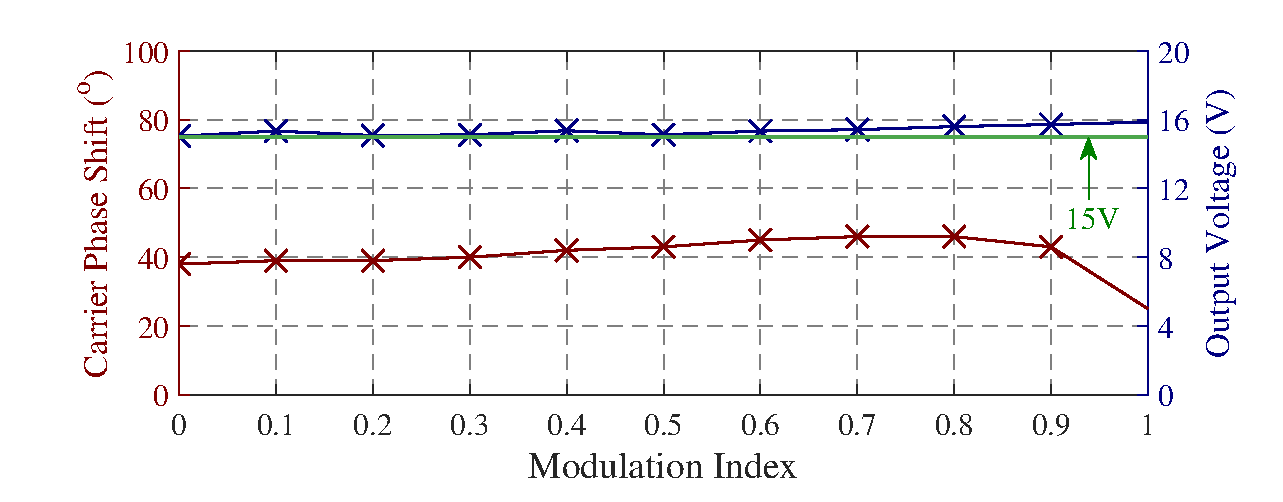
\includegraphics[width=1\linewidth]{look_up_table_v2.eps}}
\subfigure[Switching frequencies to reach 15 V output for varying modulation indices.]{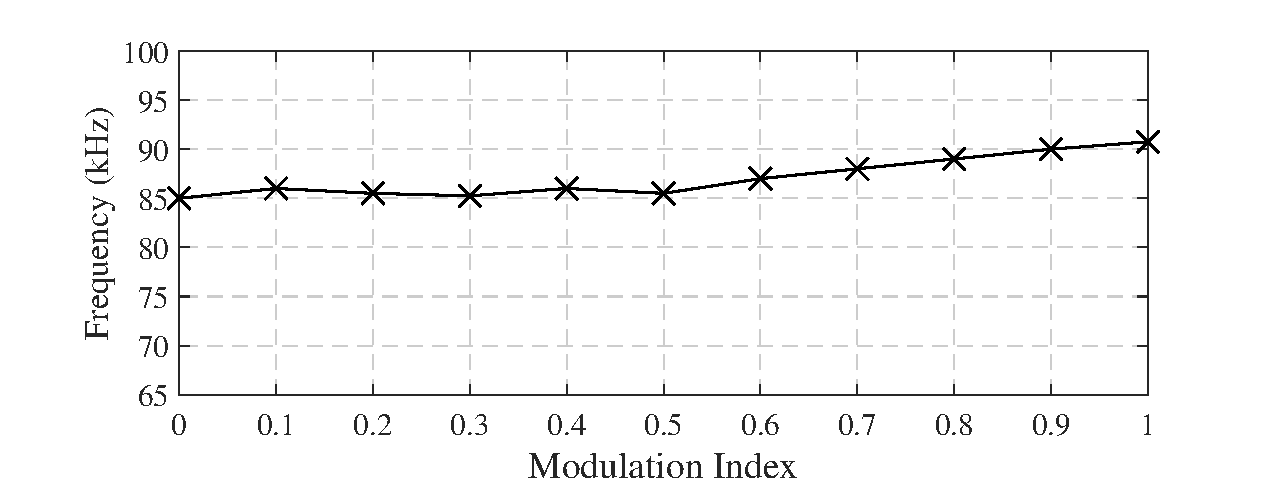
\includegraphics[width=1\linewidth]{frequency_detuning.eps}} 
\caption{Embedding look-up table and frequency detuning method.} 
    \label{fig:look_up_table_exp}
\end{figure}
%%%%%%%%%%%

\vspace*{-4mm}
\section{Comparison with Existing Studies}
Existing multi-frequency WPT systems in the literature are given in Table \ref{tab:comparison_literature}.
The proposed method provides independent control of the dual-band output voltage.
Unlike~\cite{programmablePWM}, it is not  required completely offline calculation where it is not possible to apply dynamic applications like motor drive systems. Although a look-up table is embedded in the proposed system to control the switching frequency and its sideband components, conventional online modulation techniques still achieve the low-frequency modulated component. 
Besides, online frequency detuning control can finely adjust the switching frequency and its sideband components.

In the proposed system, only low-frequency modulated motor's current is obtained by SPWM, and the WPT system directly utilizes the switching harmonics. 
Therefore, the required switching frequency of the proposed WPT system is lower than the studies given in \cite{MFML-hybrid,MFMA-circuit}.
If WPT operates at the modulated frequency rather than the switching frequency, the switching losses increase to achieve the same coil sizes. 
Thus, directly utilizing the switching frequency is significant to make the system feasible. 
In~\cite{multifreq}, switching harmonics are directly utilized, but, unlike the proposed system, it does not have an independent control method, and just a single load is supplied.
In~\cite{single-Tx}, two converters are used to achieve a dual channel using switching harmonics, while the proposed method uses only a single converter.
In~\cite{ML-inverter}, multi-frequency components are obtained by increasing the level of the converter; therefore, a higher number of switches is used than the proposed method, which increases the cost and complexity.
%%%%%%%%%
 \vspace*{-2mm}
\begin{table}[h!]
\centering
\caption{Comparison with existing studies in the literature.}
\begin{tabular}{c|c|c|c|c}
\textbf{}                                                    & \textbf{\begin{tabular}[c]{@{}c@{}}Transfer\\ Channels\end{tabular}} & \textbf{\begin{tabular}[c]{@{}c@{}}Converter\\ Numbers (Tx)\end{tabular}} & \textbf{\begin{tabular}[c]{@{}c@{}}Offline \\ Algorithm\end{tabular}} & \textbf{\begin{tabular}[c]{@{}c@{}}Operating\\ Frequency\end{tabular}} \\ \hline
\textbf{\cite{multifreq}}                                                  & 1                                                                    & 1-2LC                                                                           & Not Required          & $\geq f_s$                                                                    \\ \hline
\textbf{\cite{single-Tx}}                                                   & 2                                                                    & 2-2LC                                                                            &Not Required    &           $f_s$                                                                  \\ \hline
\textbf{\cite{programmablePWM}}                                                   & 2                                                                    & 1-2LC                                                                            & Required                                                            & $\leq f_s$                                                                     \\ \hline
\textbf{\cite{MFML-hybrid}}                                                 &            2                                                           & 1-2LC                                                                          & Not Required               & $<f_s$                                                                   \\ \hline

\textbf{\cite{MFMA-circuit}}                                                  & 4                                                                    & 1-2LC                                                                            &Not Required                & $<f_s$                                                                    \\ \hline
\textbf{\cite{ML-inverter}}                                                 &            2                                                           & 1-MLI                                                                      & Not Required               & $\geq f_s$                                                                   \\ \hline

\textbf{\begin{tabular}{c}
     This \\ Work
\end{tabular} }& 2                                                                    & 1-2LC                                                                      & 
    Not required* 
     &  $ = f_s$                                                                    \\ 
\hline


\end{tabular}
\label{tab:comparison_literature}

\begin{flushleft}
  \item \textbf{2LC} : Two level converter, \textbf{MLI} : Multi level inverter.
  % \item \textbf{ML} : Multi level converter.
  \item \textbf{*} :  A partially look-up table is required.
 \end{flushleft}
\end{table}
%%%%%%%%%
\vspace*{-8mm}
\section{Discussion}
\subsection{Current Modulation Techniques of Conventional Drives}
Many modulation techniques such as Sinusoidal PWM (SPWM), Space Vector PWM (SVPWM), and Discontinuous PWM (DPWM) are used in industrial motor drives.
Each modulation technique has its advantages.
For example, while SVPWM effectively utilizes the DC link voltage, DPWM provides reduced switching losses. 
Although the proposed system is implemented with SPWM, it can also be applied with other modulation techniques.
The change in the magnitude of the switching frequency over modulation indices is presented in Fig.~\ref{fig:SVPWM} for SPWM and SVPWM. 
It is observed that the tendency of the switching harmonic magnitude of SVPWM is similar to SPWM, and it can be controlled in line-to-line connection via the proposed CPS, as presented before.   
\begin{figure}[h!]
    \centering
    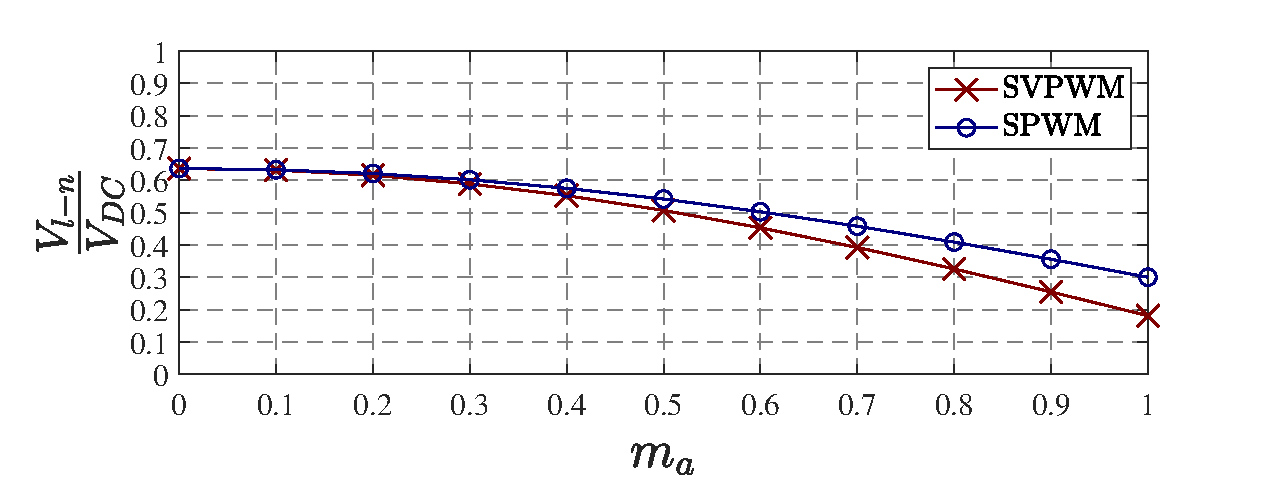
\includegraphics[width=1\linewidth]{SVPWM3.eps}
    \caption{The normalized inverter voltage ($\dfrac{V_{l-n}}{V_{DC}}$) of the switching harmonics over modulation indices ($m_a$).}
    \label{fig:SVPWM}
\end{figure}
%%%%%%%%%%

\vspace*{-6mm}
\subsection{Carrier Phase Shift Impacts on the Motor}
In the conventional SPWM method, the switching frequency components are not observed in line-to-line voltages, and the magnitudes of the sideband harmonics increase by the modulation index. 
However, in the proposed method, the switching component is controlled by the carrier phase shift and so is also observed in line-to-line voltages.
The effective voltages, which are calculated as in (\ref{eq:equ_cent}), are plotted in Fig. \ref{fig:W/outCar} for with and without carrier phase shift method. 
%%%%%%%%%
It is observed that the effective voltage harmonics in the proposed system are greater than the conventional SPWM until $m_a$ reaches~0.9. 
However, the harmonics attenuate in motor phase currents thanks to large motor phase inductances. Since the voltage harmonic at the fundamental frequency (low-frequency modulated signal of the SPWM) is not affected by the carrier phase shift and high-frequency components are filtered out, the motor operation and efficiency do not significantly change with the proposed method. 
However, if a low-inductance motor is used or the switching period is not short enough compared to the motor's time constant ( depending on motor phase inductances and resistances), the voltage harmonics also produce harmonics in motor phase currents. 
In this condition,  introducing carrier-phase shift generates high-frequency current ripples, which creates torque ripple and decreases the efficiency.  
Therefore, the switching frequency should be selected considering the motor electrical time constant to avoid current harmonics due to the carrier phase shift.
%%%%%%%
\vspace*{-3mm}
\begin{figure}[h!]
    \centering
    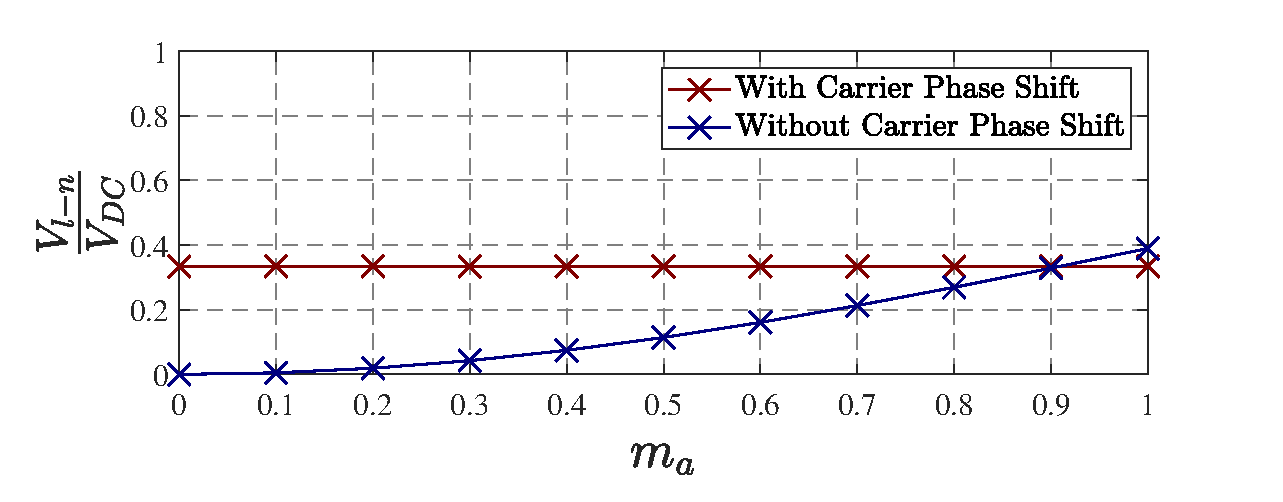
\includegraphics[width=1\linewidth]{CPS_impact.eps}
    \caption{The the effective inverter voltage ($\dfrac{V_{l-n}}{V_{DC}}$) for the switching harmonic and it sidebands over modulation indices ($m_a$).}
    \label{fig:W/outCar}
\end{figure}

\vspace*{-6mm}
\subsection{Low-Frequency Fluctuation on the Output Voltage}
Rectified sideband harmonic components generate low-frequency ripples (at the double-fundamental and quad-fundamental frequencies) even though they contribute to the DC output voltage. 
The WPT system cannot filter out these sideband harmonic components since they are close to the switching frequency. 
Besides, the magnitude of the low-frequency ripples increases for a higher modulation index since sideband components become more dominant with the increased modulation index.
The variations of low-frequency current components with changing modulation indices are shown in Fig. \ref{fig:low_freq}. 
\vspace*{-2mm}
%%%%%%%%%
\begin{figure}[h!]
    \centering
    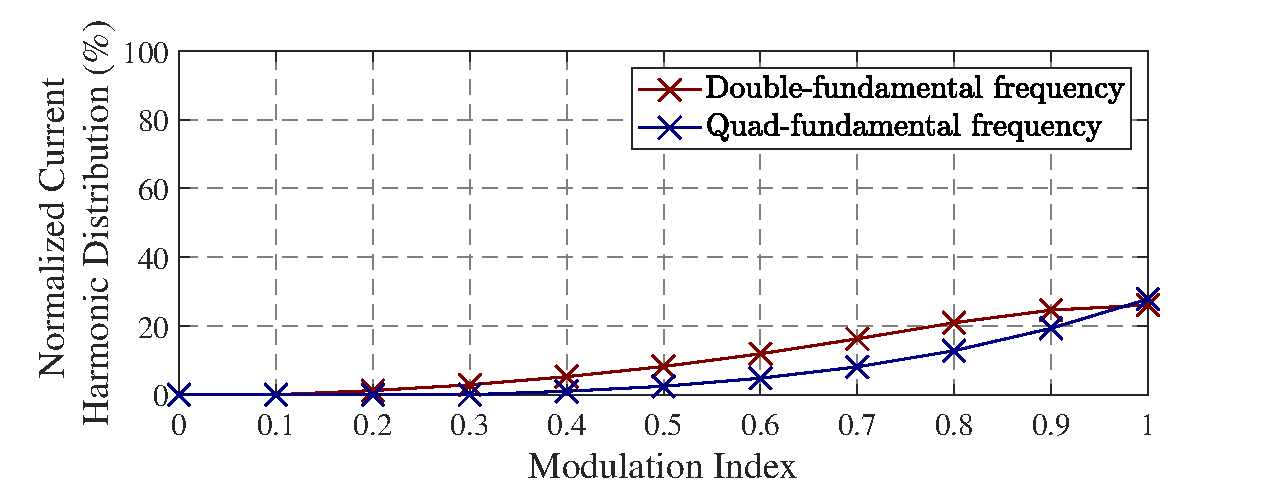
\includegraphics[width=1\linewidth]{low_frequeny_ripple.eps}
    \caption{The ratio of the low-frequency harmonic components in the rectifier current over modulation indexes ($m_a$)}
    \label{fig:low_freq}
\end{figure}
\vspace*{-2mm}
\begin{equation}
\Delta V =\Delta t_2 \frac{\Delta I_2}{C_{OUT}}+\Delta t_4 \frac{\Delta I_4}{C_{OUT}}
\label{eq:output_cap}
\end{equation}
% \vspace{-6mm}
These current ripples can be easily filtered out in the output voltage by adding output capacitance. 
Peak-to-peak voltage fluctuation can be calculated as in (\ref{eq:output_cap}), where $C_{OUT}$ is the output capacitance, $\Delta t_2$ and $\Delta t_4$  are the periods of double-fundamental and quad-fundamental frequencies, $\Delta I_2$ and $\Delta I_4$ are the peak-to-peak values at $m_a=1$ under rated load. 
Therefore, the voltage fluctuation can be brought to the desired value by adding appropriate output capacitance.

\vspace{-2mm}
%%%%%%%
%%%%%%%
\subsection{Effect of Switching Frequency and Type of Semiconductors}
Several factors should be considered while selecting the switching frequency.  
Firstly, a higher switching frequency shrinks the coil size but increases eddy losses, which can be reduced with Litz wires.
Secondly, the inverter voltage harmonics create motor current ripples, which can be decreased by increasing the switching frequency.
Since the proposed carrier phase shift method also has a negative effect on voltage harmonics, the switching frequency should be selected carefully.
However, the upper limit for the switching frequency is usually dictated by the motor drive.
In conventional silicon (Si)-based motor drives, the switching frequency is usually around 20 kHz \cite{motor_si-based}.
At these frequencies, Tx-Rx coils get bulky, and motor current ripple (especially for high-speed motors with higher fundamental frequency) increases. 
Therefore, implementing the proposed system with conventional Si-based motor drives is challenging. 
On the other hand, wide bandgap (WBG) based motor drives (such as silicon carbide (SiC) or gallium nitride (GaN)) are becoming more popular with recent advancements in semiconductor technology.
They can provide higher switching frequencies (up to several hundred kHz) without sacrificing efficiency~\cite{gan_drive,gan_driver2}.
Thus, with WBG-based motor drives,  a sweet spot in the switching frequency can be found that makes the proposed method feasible by reducing the coil size and current ripple.
\vspace*{-2mm}
%%%%%%%%
\section{Conclusion}
%\vspace*{-2mm}
This paper proposes a concurrent dual-frequency power transfer method for wired and wireless systems using just a single inverter.
The proposed method can reduce the system cost and size for applications that require power transfer to rotating frames, such as rotating sensors, radars, and auxiliary systems.
This study also presents a novel carrier phase shift~(CPS) method to regulate the power transferred to the WPT systems.
Therefore, active converters on the Rx side are not required, which reduces the complexity and weight of the system on the rotating frame.
However, a few concerns reveal in selecting switching frequency. 
On the one hand, the switching frequency should be high enough to avoid the impact of the CPS method on the motor phase currents and make WPT coils' size feasible. On the other hand, the upper limit of the switching frequency is dictated by the motor drive due to losses. 
WBG-based motor drives, which are the trend in industrial motor drives,  help to find a sweet spot in the switching frequency considering all these concerns.
In order to validate the proposed system, an experimental setup with a GaN-based drive was established.  
It was acquired that the switching harmonic and the fundamental
frequency is controlled independently by the proposed CPS method.
However, it was observed that the measured output voltage deviates from theoretical calculations due to high-order harmonics and the effect of parasitics or nonidealities, so the frequency detuning method is proposed to compensate for these deviations.
It is also acquired that low-frequency ripple at the output exists due to sideband harmonics, and this ripple can easily be filtered out using proper output capacitance.


\bibliographystyle{IEEEtran}
%\vspace*{-4mm}
\bibliography{ref.bib}
\vspace{-4mm}
\begin{IEEEbiography}[{
\includegraphics[width=1\linewidth]{enes1.jpg}}]
{Enes Ayaz} received the B.Sc. degree from the Department of Electrical and Electronics Engineering, Middle East Technical University (METU), Ankara, Turkey, in 2019, where he is currently pursuing the M.Sc. degree.

His current research interests include resonant converters, wireless power transfer, and power electronics.
\end{IEEEbiography}
% \vspace*{-130mm}
\begin{IEEEbiography}[{
\includegraphics[width=1\linewidth ]{ogunaltun1.png}}]
{Ogün Altun} received his B.Sc degree from the Department of Electrical and Electronics Engineering, Middle East Technical University, Ankara, Turkey, in 2020. He is pursuing his M.Sc. degree at Middle East Technical University. 

His current research interests are power converters, renewable energy, and wireless power transfer.
\end{IEEEbiography}
% \vspace*{-130mm}
\begin{IEEEbiography}[{
\includegraphics[width=1\linewidth ]{ozan.png}}]
{Ozan Keysan} received the master’s degree from Middle East Technical University (METU), Ankara, Turkey, in 2008, and the Ph.D. degree from The University of Edinburgh, Edinburgh, U.K., in 2014. 

He is currently an Associate  Professor with the Department of Electrical and Electronics Engineering, METU. 
His current research interests include wireless power transfer, renewable energy, design and optimization of electrical machines, smart grids, superconducting machines, and permanent-magnet machines.
\end{IEEEbiography}

% \appendi

\end{document}


